\documentclass{article}\usepackage[]{graphicx}\usepackage[]{color}
%% maxwidth is the original width if it is less than linewidth
%% otherwise use linewidth (to make sure the graphics do not exceed the margin)
\makeatletter
\def\maxwidth{ %
  \ifdim\Gin@nat@width>\linewidth
    \linewidth
  \else
    \Gin@nat@width
  \fi
}
\makeatother

\definecolor{fgcolor}{rgb}{0.345, 0.345, 0.345}
\newcommand{\hlnum}[1]{\textcolor[rgb]{0.686,0.059,0.569}{#1}}%
\newcommand{\hlstr}[1]{\textcolor[rgb]{0.192,0.494,0.8}{#1}}%
\newcommand{\hlcom}[1]{\textcolor[rgb]{0.678,0.584,0.686}{\textit{#1}}}%
\newcommand{\hlopt}[1]{\textcolor[rgb]{0,0,0}{#1}}%
\newcommand{\hlstd}[1]{\textcolor[rgb]{0.345,0.345,0.345}{#1}}%
\newcommand{\hlkwa}[1]{\textcolor[rgb]{0.161,0.373,0.58}{\textbf{#1}}}%
\newcommand{\hlkwb}[1]{\textcolor[rgb]{0.69,0.353,0.396}{#1}}%
\newcommand{\hlkwc}[1]{\textcolor[rgb]{0.333,0.667,0.333}{#1}}%
\newcommand{\hlkwd}[1]{\textcolor[rgb]{0.737,0.353,0.396}{\textbf{#1}}}%

\usepackage{framed}
\makeatletter
\newenvironment{kframe}{%
 \def\at@end@of@kframe{}%
 \ifinner\ifhmode%
  \def\at@end@of@kframe{\end{minipage}}%
  \begin{minipage}{\columnwidth}%
 \fi\fi%
 \def\FrameCommand##1{\hskip\@totalleftmargin \hskip-\fboxsep
 \colorbox{shadecolor}{##1}\hskip-\fboxsep
     % There is no \\@totalrightmargin, so:
     \hskip-\linewidth \hskip-\@totalleftmargin \hskip\columnwidth}%
 \MakeFramed {\advance\hsize-\width
   \@totalleftmargin\z@ \linewidth\hsize
   \@setminipage}}%
 {\par\unskip\endMakeFramed%
 \at@end@of@kframe}
\makeatother

\definecolor{shadecolor}{rgb}{.97, .97, .97}
\definecolor{messagecolor}{rgb}{0, 0, 0}
\definecolor{warningcolor}{rgb}{1, 0, 1}
\definecolor{errorcolor}{rgb}{1, 0, 0}
\newenvironment{knitrout}{}{} % an empty environment to be redefined in TeX

\usepackage{alltt}
\usepackage[utf8]{inputenc}
\usepackage{amsmath}
\usepackage{graphicx}
%\usepackage{bbold}
\usepackage{tikz}
%\usepackage{silence}
\usepackage{mdframed}
%\WarningFilter{mdframed}{You got a bad break}
\usepackage[colorinlistoftodos]{todonotes}
\usepackage{listings}
\usepackage{color}
\colorlet{exampcol}{blue!10}
\usepackage{multicol}
\usepackage{booktabs}

\title{BIO311: Population Ecology\\ \textit{Practical 10:\\ Stochasticity in Matrix Models\\ Population Viability Analysis\\ \& Metapopulation Dynamics.}}
\setlength\parindent{0pt}

\setcounter{tocdepth}{1} % Determines the depth of the table of contents;; 0:chapters, 1: chapters and sections, 2: chapters,sections and subsections

%\renewcommand{\theExercise}{\thechapter.\arabic{Exercise}}%

\setlength\parindent{0pt}
\IfFileExists{upquote.sty}{\usepackage{upquote}}{}
\begin{document}

\author{Timoth\'ee Bonnet \&\footnote{This document was co-authored by Tina Cornioley}\; Koen van Benthem\\\\
\tt{timothee.bonnet@ieu.uzh.ch}\\ \tt{koen.vanbenthem@ieu.uzh.ch}}

\date{Spring 2016}



\maketitle
\tableofcontents
\vspace{3cm}

\newpage


\section{Environmental Stochasticity}
In practical $9$ we investigated the population dynamics for two populations of yellow-necked mice. Here we focus on one of the two populations presented in that practical: the population living on the plain. For this population the Leslie matrix was given by:
\begin{equation*} \boldsymbol{A}=% latex table generated in R 3.2.3 by xtable 1.8-0 package
% Mon Mar 14 13:21:32 2016
\begin{pmatrix}{}
  0.00 & 2.00 \\ 
  0.25 & 0.50 \\ 
  \end{pmatrix}
\end{equation*}
It turns out however that the conditions for the population are not the same every year. Measurements have been done (okay, this is what we say, in reality we made up some numbers that give reasonable results in the end...) for three years in a row and the matrices that were found for these years are shown below:
\begin{align*}\boldsymbol{A_1} &=% latex table generated in R 3.2.3 by xtable 1.8-0 package
% Mon Mar 14 13:21:32 2016
\begin{pmatrix}{}
  0.00 & 2.00 \\ 
  0.25 & 0.50 \\ 
  \end{pmatrix}
& \boldsymbol{A_2} &=% latex table generated in R 3.2.3 by xtable 1.8-0 package
% Mon Mar 14 13:21:32 2016
\begin{pmatrix}{}
  0.00 & 2.00 \\ 
  0.27 & 0.54 \\ 
  \end{pmatrix}
& \boldsymbol{A_3} &=% latex table generated in R 3.2.3 by xtable 1.8-0 package
% Mon Mar 14 13:21:32 2016
\begin{pmatrix}{}
  0.00 & 1.80 \\ 
  0.20 & 0.44 \\ 
  \end{pmatrix}
\\ \lambda &= 1 &\lambda &= 1.052879 &\lambda &= 0.8590618\end{align*}
We see that the year that we considered was a relatively average year. The year after the survival rates of the individuals was higher at both stages. In the third year however the population experienced some severe conditions with the survival rates and the fertility rate being lower than in both preceding years.

We thus have to realise that the transition rates in nature will vary from year to year. This would mean that the Leslie matrix would also look differently every year. Two possibilities of taking this into account when predicting the behaviour of the population are given below:
\begin{enumerate}
\item From the matrices we see that the mean fertility rate is $\mu_{F} = 1.9333333$ with a standard deviation of $\sigma_{F} = 0.1154701$. For the survival rates we find:
\begin{align*}
\mu_{S_j} &= 0.24 & \sigma_{S_j} &= 0.0360555\\
\mu_{S_a} &= 0.4933333 & \sigma_{S_a} &= 0.0503322
\end{align*}
For every time step that we project the population in the future, we generate a matrix $\boldsymbol{A}$ with a random fertility rate (drawn from a normal distribution with mean $\mu_F$ and standard deviation $\sigma_F$), a random juvenile survival rate (drawn from a normal distribution with mean $\mu_{S_j}$ and standard deviation $\sigma_{S_j}$) and a random adult survival rate (drawn from a normal distribution with mean $\mu_{S_a}$ and standard deviation $\sigma_{S_a}$). This way we will incorporate the fact that the rates can vary over time.
\begin{mdframed}
\textbf{Quick refresher: standard deviation}\\
The standard deviation describes how much variation there is in the data from the average. A large standard deviation means that the data points deviate a lot from the average whereas a small standard deviation indicates that the data points are close to the average. Mathematically it is defined as:
\begin{equation*}
\sigma = \sqrt{\frac{1}{N-1}\sum_{i=1}^{N}{(x_i-\mu)^2}}.
\end{equation*}
In this equation $\mu$ is the average value of $x$ (thus $\mu=\frac{1}{N}\sum_{i=1}^{N}{x_i}$) and $N$ is the total number of data points. In \texttt{R} you can use the function \texttt{sd()} to calculate the standard deviation.
\end{mdframed}
\item Every time step we randomly choose one of the measured matrices ($\boldsymbol{A_1,A_2,A_3}$) with equal probabilities. Thereby taking into account the variation in the environment.
\end{enumerate}
Which of these approaches do you prefer in this case? And why?
\subsection{Independent sequences}
In the rest of this practical, we will explore what happens if we decide to model the dynamics by randomly choosing one of the three matrices each time step. Assume an initial population of $5$ juveniles and $5$ adults. Create a matrix \texttt{N} to store the numbers that you will calculate. Now use the \texttt{sample()} function to generate a random number every time step and use this number (using \texttt{if/else}) to decide which matrix is used in a specific time step. To illustrate the use of \texttt{sample}
\begin{knitrout}
\definecolor{shadecolor}{rgb}{0.969, 0.969, 0.969}\color{fgcolor}\begin{kframe}
\begin{alltt}
\hlkwd{sample}\hlstd{(}\hlkwd{c}\hlstd{(}\hlnum{1}\hlstd{,}\hlnum{2}\hlstd{,}\hlnum{3}\hlstd{,}\hlnum{4}\hlstd{),}\hlnum{1}\hlstd{)}
\end{alltt}
\begin{verbatim}
## [1] 1
\end{verbatim}
\end{kframe}
\end{knitrout}
randomly draws $1$ entry out of the vector \texttt{c(1,2,3,4)}. Now use this function to generate one possible prediction of the population dynamics until time step $50$.
\begin{knitrout}
\definecolor{shadecolor}{rgb}{0.969, 0.969, 0.969}\color{fgcolor}\begin{kframe}
\begin{alltt}
\hlstd{A1}\hlkwb{<-}\hlstd{...}
\hlstd{A2}\hlkwb{<-}\hlstd{...}
\hlstd{A3}\hlkwb{<-}\hlstd{...}

\hlstd{timesteps}\hlkwb{<-}\hlstd{...} \hlcom{# Total number of timesteps}

\hlstd{N}\hlkwb{<-}\hlstd{...} \hlcom{# Create matrix to store the calculated values}
\hlstd{N[,}\hlnum{1}\hlstd{]}\hlkwb{<-}\hlstd{...}

\hlkwa{for}\hlstd{(t} \hlkwa{in} \hlstd{...)\{}

  \hlstd{test}\hlkwb{<-}\hlstd{.....} \hlcom{# Use sample to generate }
              \hlcom{# a random number (1,2,3)}

  \hlkwa{if}\hlstd{(test}\hlopt{==}\hlstd{..)\{}
    \hlstd{...}
  \hlstd{\}}\hlkwa{else if}\hlstd{(test}\hlopt{==}\hlstd{...)\{}
    \hlstd{...}
  \hlstd{\}}\hlkwa{else}\hlstd{\{}
    \hlstd{...}
  \hlstd{\}}
\hlstd{\}}
\hlstd{Ntot}\hlkwb{<-}\hlkwd{colSums}\hlstd{(N)}  \hlcom{# Calculate total population size}
                  \hlcom{# per timestep}

\hlkwd{plot}\hlstd{(...)}
\end{alltt}
\end{kframe}
\end{knitrout}

\begin{knitrout}
\definecolor{shadecolor}{rgb}{0.969, 0.969, 0.969}\color{fgcolor}

{\centering 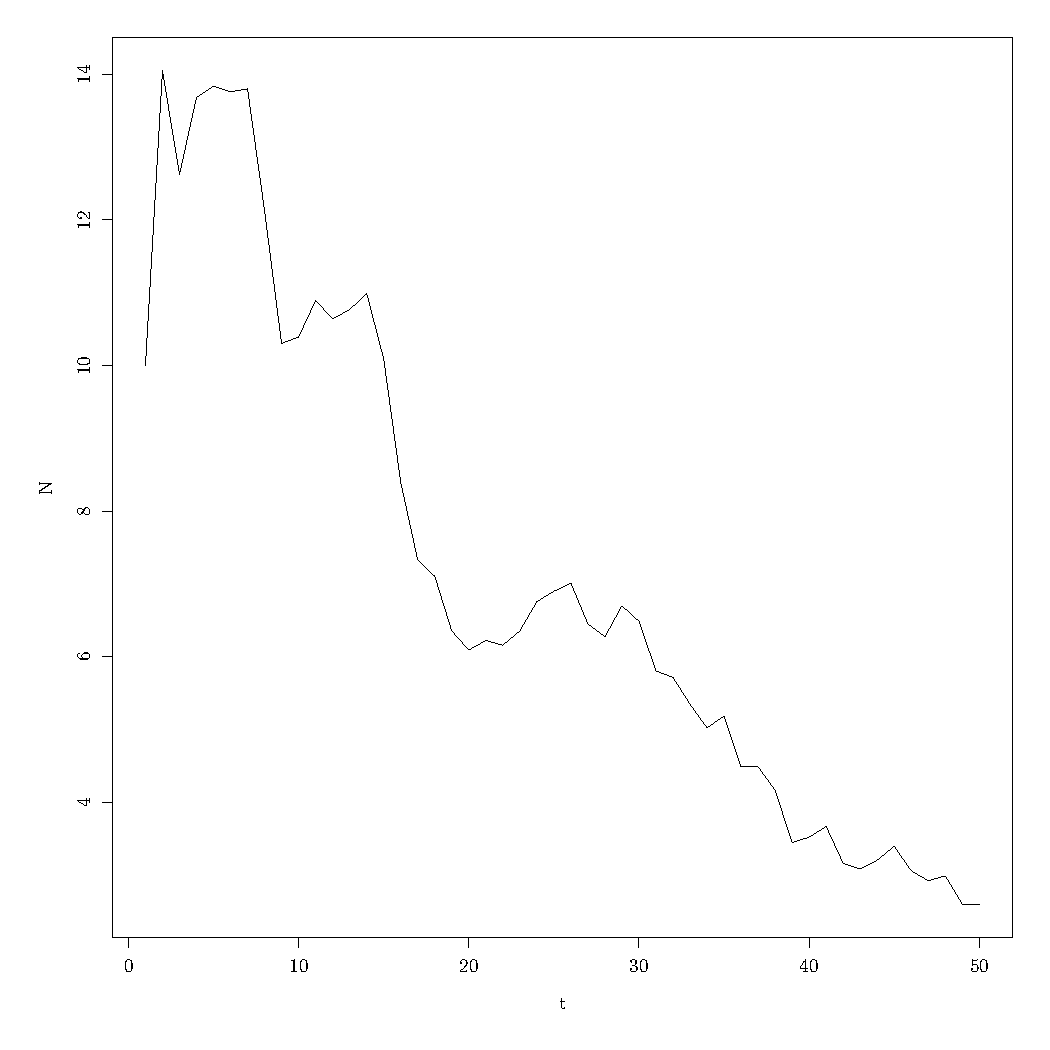
\includegraphics[width=0.5\textwidth]{figure/sim_one-1} 

}



\end{knitrout}

You will probably notice that your result looks different from the result in the graph above. The reason for this is that the outcome depends on random numbers. It is actually not really interesting to see what one prediction tells us. Instead, write a loop that repeats the whole prediction multiple times (for example $200$ times) and plot the results of all these predictions in one graph. For this it is best to start with an empty plot and add the different realisations using the \texttt{lines()} function (see practical 7, page 20 where we used a similar approach for stochasticity in the logistic growth model). In English, what we want to do is:

\begin{enumerate}
\item Define the number of different simulations (replicates) that you want to perform
\item Create an empty plot
\item Run one of the simulations\label{steppie}
\item Use \texttt{lines()} to add a line with that outcome to the plot. Use the argument \texttt{col} to specify a color for this line. If you want to automatically generate a large number of different colors, take a look at the function \texttt{rainbow()}.
\item If you have not yet done all the simulations, return to step \ref{steppie}
\end{enumerate}
The more lines you draw on one plot, the more complicated the interpretation of the plot becomes. In order to make the interpretation a bit easier, we recommend drawing a line that corresponds to the average behaviour of all the lines. To do so, we create a vector \texttt{TotalN} at the beginning of the code (before the loops) that first contains only zeros:
\begin{knitrout}
\definecolor{shadecolor}{rgb}{0.969, 0.969, 0.969}\color{fgcolor}\begin{kframe}
\begin{alltt}
\hlstd{TotalN}\hlkwb{<-}\hlkwd{rep}\hlstd{(}\hlnum{0}\hlstd{,timesteps)}
\end{alltt}
\end{kframe}
\end{knitrout}
at the end of the calculation of each simulation we have the vector \texttt{Ntot} that contains the simulated number of individuals at each time step. (In \texttt{Ntot}, \texttt{tot} refers to the fact that it is both the juveniles and the adults. In \texttt{TotalN}, \texttt{Total} refers to the fact that this vector contains the sum of all the different predictions), we add that line to \texttt{TotalN}:
\begin{knitrout}
\definecolor{shadecolor}{rgb}{0.969, 0.969, 0.969}\color{fgcolor}\begin{kframe}
\begin{alltt}
\hlstd{TotalN}\hlkwb{<-}\hlstd{TotalN}\hlopt{+}\hlstd{Ntot}
\end{alltt}
\end{kframe}
\end{knitrout}
Finally, after having calculated all the different predictions, divide \texttt{TotalN} by the number of predictions to obtain the main behaviour. You can add this behaviour to the plot with \texttt{lines()} after the calculations have been finished. Change the \texttt{lwd} parameter to draw a thicker (more visible) line and the colour with \texttt{col=} to be able to distinguish the line. What is the trend of this average line? Is this what you expected based on the initial matrices? 





\subsection{Temporal environmental correlations}
So far we have assumed that the chances of applying either matrix ($\boldsymbol{A_1,A_2,A_3}$) is the same. In some cases however, the conditions experienced by a population vary slowly: It is more likely that a population is exposed to similar conditions at the next time step compared to the current time step than to different conditions. In terms of matrices, this means that if at time $t$ matrix $\boldsymbol{A_1}$ is applied, it is more likely that at the next time step the same matrix is applied than that one of the other ones is used. As an example you can think of copper pollution: this pollution is expected to last multiple years, so if there is pollution this year, there will probably still be some pollution next year. Assume for example that matrix $\boldsymbol{A_3}$ describes the dynamics of the population in case of copper pollution and the population experiences this pollution at a time $t$. In this case we expect the copper pollution to still be there at time $t+1$ and therefore we assume that the chance of applying $\boldsymbol{A_3}$ at time step $t+1$ should be larger than the chance of applying one of the other two matrices that describe good conditions.

You will now incorporate this property in the model that you have already developed. The \texttt{sample()} function can be given a parameter \texttt{prob} that specifies the probability of drawing a specific number. Try this by repeatedly performing the following line:
\begin{knitrout}
\definecolor{shadecolor}{rgb}{0.969, 0.969, 0.969}\color{fgcolor}\begin{kframe}
\begin{alltt}
\hlkwd{sample}\hlstd{(}\hlkwd{c}\hlstd{(}\hlnum{1}\hlstd{,}\hlnum{2}\hlstd{,}\hlnum{3}\hlstd{),}\hlnum{1}\hlstd{,}\hlkwc{prob}\hlstd{=}\hlkwd{c}\hlstd{(}\hlnum{4}\hlopt{/}\hlnum{7}\hlstd{,}\hlnum{2}\hlopt{/}\hlnum{7}\hlstd{,}\hlnum{1}\hlopt{/}\hlnum{7}\hlstd{))}
\end{alltt}
\end{kframe}
\end{knitrout}
Now you can use this property to change the previous simulation to account for temporal auto-correlation. First, before entering the time loop (but after entering the loop that is used for calculating the different predictions), specify a new vector that will hold the probabilities. At this time (the first time point), all the matrices are still equally likely to occur.
\begin{knitrout}
\definecolor{shadecolor}{rgb}{0.969, 0.969, 0.969}\color{fgcolor}\begin{kframe}
\begin{alltt}
\hlstd{probs}\hlkwb{=}\hlkwd{c}\hlstd{(}\hlnum{1}\hlopt{/}\hlnum{3}\hlstd{,}\hlnum{1}\hlopt{/}\hlnum{3}\hlstd{,}\hlnum{1}\hlopt{/}\hlnum{3}\hlstd{)}
\end{alltt}
\end{kframe}
\end{knitrout}
Now adapt your previous code to use these probabilities to draw a new matrix every time step. Once a matrix has been drawn in a time step, change the vector \texttt{probs} such that the next time step there will be a chance of $\frac{5}{7}$ to have the same matrix again and a chance of $\frac{1}{7}$ to have either of the other matrices in the next time step. In English, what you have to do is:

\begin{enumerate}
\item Define a \texttt{probs} vector within the first loop but outside of the second. This is the vector that determines which one of the matrix is the first matrix of the time step.
\item Specify the \texttt{prob} argument of the \texttt{sample} function to be the vector \texttt{probs}.
\item After each \texttt{if/else} statements within the second loop, define a new \texttt{probs} vector which will change the probability of the matrices to be used.
\end{enumerate}
How do these predictions differ from the predictions in the non-correlated case? Does this make sense to you?

\section{Population Viability Analysis}
What managers want to know generally is not so much the average prediction, but rather the chance of extinction. What is the chance that this population will go extinct in the next $50$ year? In order to look into this, we first need to define 'extinct': with the matrix models the vectors will never really reach $0$, but they can become really small (say a total population size of $0.001$). We thus need to decide when we call a population extinct. In this case we decide that if the population contains less than $2$ individuals, it basically went extinct. If the population size falls below this threshold, we do not actually multiply the population by the matrix, but we just set the new value of the population vector to be $\begin{pmatrix} 0 \\ 0 \end{pmatrix}$. To make the code easier to adapt, we first define a threshold variable:
\begin{knitrout}
\definecolor{shadecolor}{rgb}{0.969, 0.969, 0.969}\color{fgcolor}\begin{kframe}
\begin{alltt}
\hlstd{threshold}\hlkwb{<-}\hlnum{2}
\end{alltt}
\end{kframe}
\end{knitrout}
Now within the second loop and before the other statements, add an \texttt{if} statement to your code to account for this possibility. You want that if the total population size at the former time step is below the threshold, the current population size is set to $0$. 

Finally we would like to keep track of the number of extinctions over time. In order to so, create a vector \texttt{extinct} at the beginning of your code, before entering any loop:
\begin{knitrout}
\definecolor{shadecolor}{rgb}{0.969, 0.969, 0.969}\color{fgcolor}\begin{kframe}
\begin{alltt}
\hlstd{extinct}\hlkwb{<-}\hlkwd{rep}\hlstd{(}\hlnum{0}\hlstd{,timesteps)}
\end{alltt}
\end{kframe}
\end{knitrout}
Now adapt your code such that if the population size of a specific prediction at some point in time falls below the threshold, not only the population vector is set to $\begin{pmatrix} 0 \\ 0 \end{pmatrix}$, but also the extinction is counted, that is that in that case:
\begin{knitrout}
\definecolor{shadecolor}{rgb}{0.969, 0.969, 0.969}\color{fgcolor}\begin{kframe}
\begin{alltt}
\hlstd{extinct[t]}\hlkwb{<-}\hlstd{extinct[t]}\hlopt{+}\hlnum{1}
\end{alltt}
\end{kframe}
\end{knitrout}
At the end, to find the proportion of predictions that has gone extinct, you just have to divide the vector \texttt{extinct} by the number of predictions that it is based on. If this number is large enough, the proportion of extinct predictions is the probability of extinction for that population. Implement this in the code after the loops and plot how the probability of extinction changes over time. What happens if your initial population is smaller? (for example 2 adults and 2 juveniles) What is the difference in extinction probabilities between the case of time correlated environments and time uncorrelated environments? Does this make sense to you?

If you start with a population of 5 adults and 5 juveniles and make 200 simulations, your (average) result should look similar to the following graphs (in time uncorrelated environments):
\begin{center}
\begin{tabular}{c c}

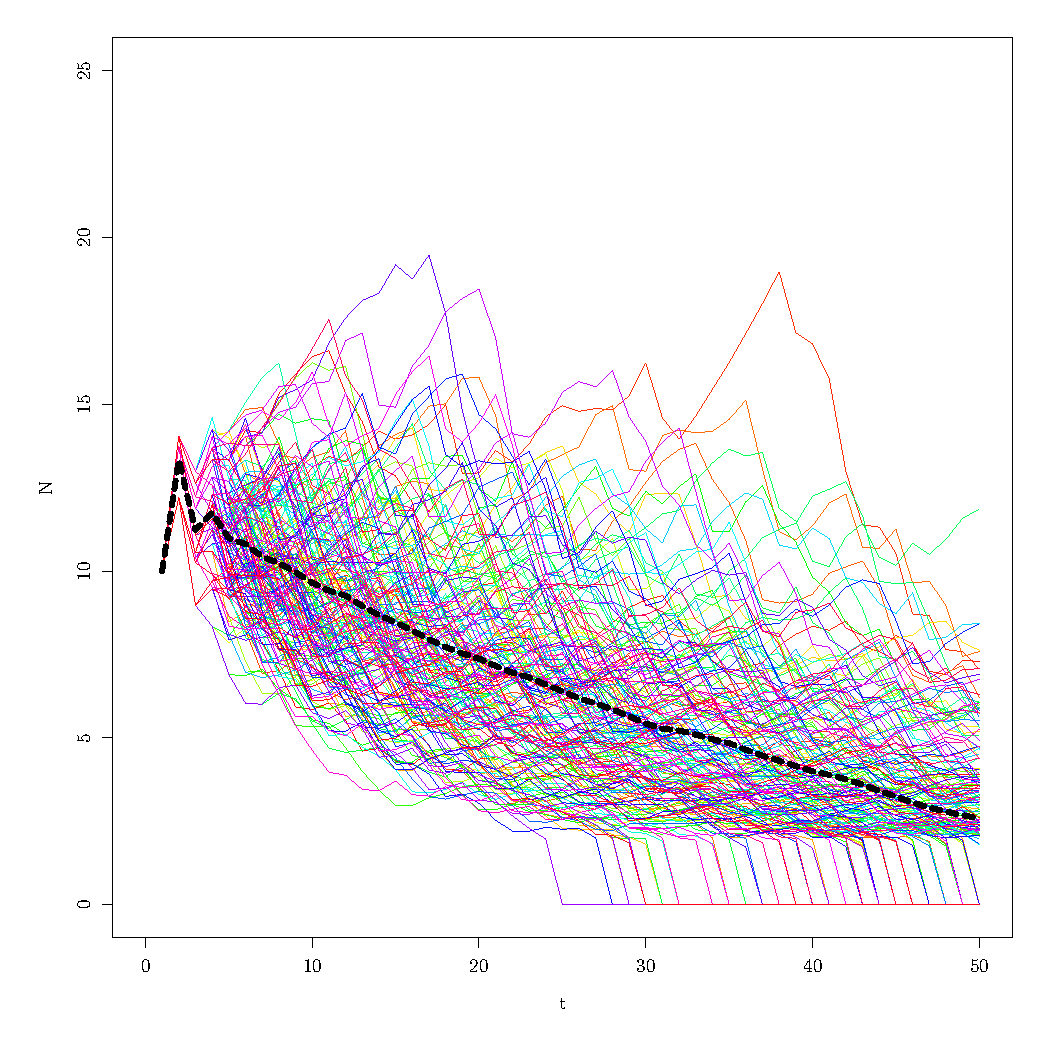
\includegraphics[width=0.40\textwidth]{figure/simop-1} 
 & 
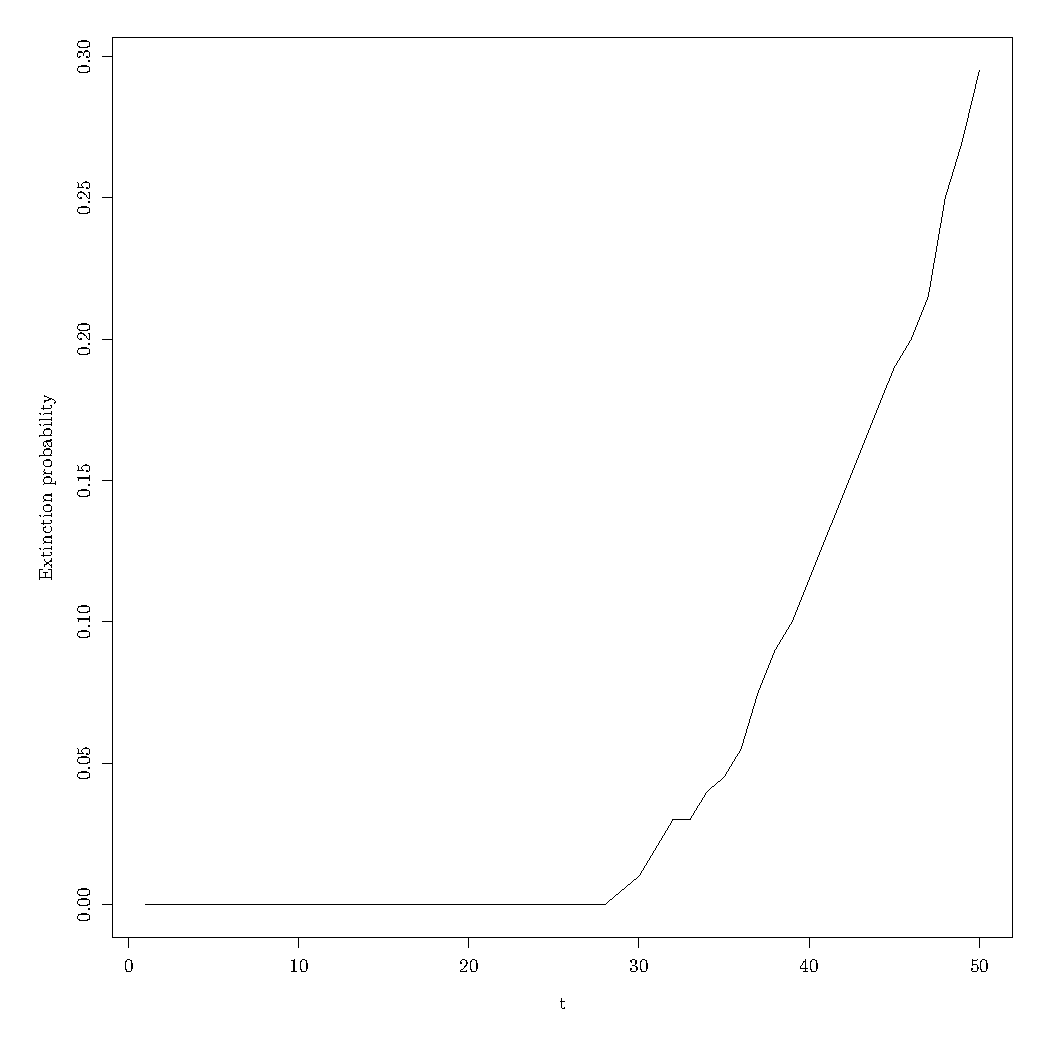
\includegraphics[width=0.40\textwidth]{figure/simop-2} 

\end{tabular}
\end{center}
\section{Demographic Stochasticity (Demonstration only)}
A problem that we have not talked about so far is the fact that matrices allow for half individuals. You may for example find that the expected number of juveniles after 10 time steps equals $2.4$, but what are $0.4$ individuals? We interpret this as an 'average'. It is however also possible to take into account the fact that half an individual can not exist. For this we do not use the matrix framework, but we can use the rates that we also used in the matrix framework.

In this section we will only consider $\boldsymbol{A_1}$. That is: we have juvenile survival of $0.25$, and adult survival of $0.5$ and an average fertility rate of $2$. If we would do the matrix multiplication, we would write for the number of juveniles ($N_j$) and the number of adults ($N_a$):
\begin{align*}
N_j(t+1) &= 2\cdot N_a (t)\\
N_a(t+1) &= 0.25\cdot N_j(t) + 0.5\cdot N_a(t)
\end{align*}
This will however give rise to half individuals as well.

In order to get rid of this problem we interpret the juvenile survival rate as follows: the juvenile survival rate is the chance that an individual juvenile survives. We can simulate this in \texttt{R} with the function \texttt{rbinom(n,size,prob)}. This function simulates how many times an event occurs if we make \texttt{size} attempts and the chance of an attempt succeeding is \texttt{prob}. The element \texttt{n} specifies how many simulations of this type we want to have.

For example we have a dice with 6 sides and we want to roll it $100$ times and we want to know how many of these $100$ times the number on the dice is either $1$ or $2$. The chance of rolling either a $1$ or a $2$ is $\frac{1}{6}+\frac{1}{6}=\frac{1}{3}$, so we expect this to happen $33.3333\dots$ times if we roll the dice $100$ times. Let us simulate this in \texttt{R}:
\begin{knitrout}
\definecolor{shadecolor}{rgb}{0.969, 0.969, 0.969}\color{fgcolor}\begin{kframe}
\begin{alltt}
\hlkwd{rbinom}\hlstd{(}\hlkwc{n}\hlstd{=}\hlnum{1}\hlstd{,}\hlkwc{size}\hlstd{=}\hlnum{100}\hlstd{,}\hlkwc{prob}\hlstd{=}\hlnum{1}\hlopt{/}\hlnum{3}\hlstd{)}
\end{alltt}
\begin{verbatim}
## [1] 31
\end{verbatim}
\end{kframe}
\end{knitrout}
We see that this function indeed returns us an integer number. \texttt{R} has in a sense simulated $100$ dice rolls and counted how many times the outcome was $1$ or $2$. If we let \texttt{R} simulate this experiment multiple times, we will find different outcomes:
\begin{knitrout}
\definecolor{shadecolor}{rgb}{0.969, 0.969, 0.969}\color{fgcolor}\begin{kframe}
\begin{alltt}
\hlkwd{rbinom}\hlstd{(}\hlkwc{n}\hlstd{=}\hlnum{10}\hlstd{,}\hlkwc{size}\hlstd{=}\hlnum{100}\hlstd{,}\hlkwc{prob}\hlstd{=}\hlnum{1}\hlopt{/}\hlnum{3}\hlstd{)}
\end{alltt}
\begin{verbatim}
##  [1] 33 32 25 36 22 25 30 42 34 32
\end{verbatim}
\end{kframe}
\end{knitrout}
However, if we average the outcomes of very many of these simulations, we should find back the expected $33.333\dots$:
\begin{knitrout}
\definecolor{shadecolor}{rgb}{0.969, 0.969, 0.969}\color{fgcolor}\begin{kframe}
\begin{alltt}
\hlkwd{mean}\hlstd{(}\hlkwd{rbinom}\hlstd{(}\hlkwc{n}\hlstd{=}\hlnum{10000}\hlstd{,}\hlkwc{size}\hlstd{=}\hlnum{100}\hlstd{,}\hlkwc{prob}\hlstd{=}\hlnum{1}\hlopt{/}\hlnum{3}\hlstd{))}
\end{alltt}
\begin{verbatim}
## [1] 33.346
\end{verbatim}
\end{kframe}
\end{knitrout}
We can now use this function to simulate the number of juveniles and adults that survive as follows:
(recall that \texttt{N[1,t]} describes the number of juveniles at time t and \texttt{N[2,t]} the number of adults at time t)
\begin{knitrout}
\definecolor{shadecolor}{rgb}{0.969, 0.969, 0.969}\color{fgcolor}\begin{kframe}
\begin{alltt}
\hlstd{N[}\hlnum{2}\hlstd{,t]}\hlkwb{<-}\hlkwd{rbinom}\hlstd{(}\hlkwc{n}\hlstd{=}\hlnum{1}\hlstd{,}\hlkwc{size}\hlstd{=N[}\hlnum{1}\hlstd{,t}\hlopt{-}\hlnum{1}\hlstd{],}\hlkwc{prob}\hlstd{=}\hlnum{0.25}\hlstd{)}
        \hlopt{+} \hlkwd{rbinom}\hlstd{(}\hlkwc{n}\hlstd{=}\hlnum{1}\hlstd{,}\hlkwc{size}\hlstd{=N[}\hlnum{2}\hlstd{,t}\hlopt{-}\hlnum{1}\hlstd{],}\hlkwc{prob}\hlstd{=}\hlnum{0.5}\hlstd{)}
\end{alltt}
\end{kframe}
\end{knitrout}
Now all that is left is calculating the amount of offspring that is produced at time t. One way of doing this is by drawing a number from a Poisson distribution with $\lambda=2$. The Poisson distribution is a distribution that is frequently used for count data, but it is beyond the scope of this course to treat it in detail. To draw a number from a Poisson distribution in \texttt{R}, we use the function \texttt{rpois(n,lambda)}. Here \texttt{n} specifies the number of numbers that we want to draw from the distribution and \texttt{lambda} specifies the mean of the distribution. So to draw one number we write:
\begin{knitrout}
\definecolor{shadecolor}{rgb}{0.969, 0.969, 0.969}\color{fgcolor}\begin{kframe}
\begin{alltt}
\hlkwd{rpois}\hlstd{(}\hlkwc{n}\hlstd{=}\hlnum{1}\hlstd{,}\hlkwc{lambda}\hlstd{=}\hlnum{2}\hlstd{)}
\end{alltt}
\begin{verbatim}
## [1] 3
\end{verbatim}
\end{kframe}
\end{knitrout}
Let us now check whether the mean value of many numbers drawn from a Poisson distribution is indeed close to 2:
\begin{knitrout}
\definecolor{shadecolor}{rgb}{0.969, 0.969, 0.969}\color{fgcolor}\begin{kframe}
\begin{alltt}
\hlkwd{mean}\hlstd{(}\hlkwd{rpois}\hlstd{(}\hlkwc{n}\hlstd{=}\hlnum{10000}\hlstd{,}\hlkwc{lambda}\hlstd{=}\hlnum{2}\hlstd{))}
\end{alltt}
\begin{verbatim}
## [1] 2.0304
\end{verbatim}
\end{kframe}
\end{knitrout}
Finally, let us have a look at which numbers are drawn most frequently when we use a Poisson distribution:
\begin{knitrout}
\definecolor{shadecolor}{rgb}{0.969, 0.969, 0.969}\color{fgcolor}\begin{kframe}
\begin{alltt}
\hlkwd{hist}\hlstd{(}\hlkwd{rpois}\hlstd{(}\hlkwc{n}\hlstd{=}\hlnum{1000}\hlstd{,}\hlkwc{lambda}\hlstd{=}\hlnum{2}\hlstd{),}\hlkwc{breaks}\hlstd{=}\hlnum{40}\hlstd{)}
\end{alltt}
\end{kframe}

{\centering 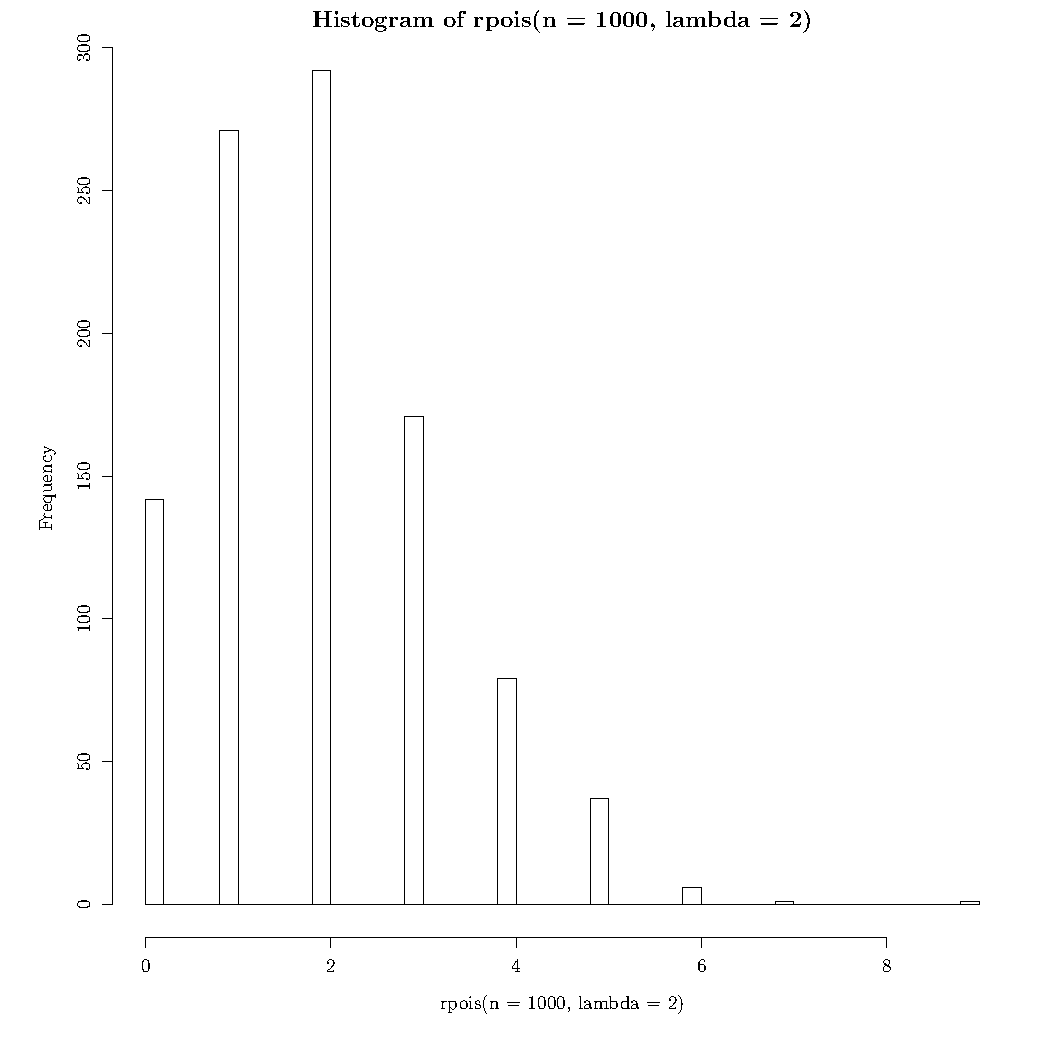
\includegraphics[width=0.5\textwidth]{figure/dice7-1} 

}



\end{knitrout}
This function would thus describe how many offspring each adult produces. If we want to know the total number of offspring produced, we can write:
\begin{knitrout}
\definecolor{shadecolor}{rgb}{0.969, 0.969, 0.969}\color{fgcolor}\begin{kframe}
\begin{alltt}
\hlstd{N[}\hlnum{1}\hlstd{,t]}\hlkwb{<-}\hlkwd{sum}\hlstd{(}\hlkwd{rpois}\hlstd{(N[}\hlnum{2}\hlstd{,t}\hlopt{-}\hlnum{1}\hlstd{],}\hlkwc{lambda}\hlstd{=}\hlnum{2}\hlstd{))}
\end{alltt}
\end{kframe}
\end{knitrout}
Let us now use this to run one simulation:
\begin{knitrout}
\definecolor{shadecolor}{rgb}{0.969, 0.969, 0.969}\color{fgcolor}\begin{kframe}
\begin{alltt}
\hlstd{timesteps}\hlkwb{<-}\hlnum{50}
\hlstd{N}\hlkwb{<-}\hlkwd{matrix}\hlstd{(}\hlnum{NA}\hlstd{,}\hlkwc{ncol}\hlstd{=timesteps,}\hlkwc{nrow}\hlstd{=}\hlnum{2}\hlstd{)}

\hlstd{N[,}\hlnum{1}\hlstd{]}\hlkwb{<-}\hlkwd{c}\hlstd{(}\hlnum{5}\hlstd{,}\hlnum{5}\hlstd{)}
\hlkwa{for}\hlstd{(t} \hlkwa{in} \hlnum{2}\hlopt{:}\hlstd{timesteps)\{}
    \hlstd{N[}\hlnum{1}\hlstd{,t]}\hlkwb{<-}\hlkwd{sum}\hlstd{(}\hlkwd{rpois}\hlstd{(N[}\hlnum{2}\hlstd{,t}\hlopt{-}\hlnum{1}\hlstd{],}\hlkwc{lambda}\hlstd{=}\hlnum{2}\hlstd{))}
    \hlstd{N[}\hlnum{2}\hlstd{,t]}\hlkwb{<-}\hlkwd{rbinom}\hlstd{(}\hlkwc{n}\hlstd{=}\hlnum{1}\hlstd{,}\hlkwc{size}\hlstd{=N[}\hlnum{1}\hlstd{,t}\hlopt{-}\hlnum{1}\hlstd{],}\hlkwc{prob}\hlstd{=}\hlnum{0.25}\hlstd{)}
        \hlopt{+} \hlkwd{rbinom}\hlstd{(}\hlkwc{n}\hlstd{=}\hlnum{1}\hlstd{,}\hlkwc{size}\hlstd{=N[}\hlnum{2}\hlstd{,t}\hlopt{-}\hlnum{1}\hlstd{],}\hlkwc{prob}\hlstd{=}\hlnum{0.5}\hlstd{)}
\hlstd{\}}
\hlstd{Ntot}\hlkwb{<-}\hlkwd{colSums}\hlstd{(N)}
\hlkwd{plot}\hlstd{(}\hlnum{1}\hlopt{:}\hlstd{timesteps,Ntot,}\hlkwc{type}\hlstd{=}\hlstr{"l"}\hlstd{,}\hlkwc{xlab}\hlstd{=}\hlstr{"t"}\hlstd{,}\hlkwc{ylab}\hlstd{=}\hlstr{"N"}\hlstd{)}
\end{alltt}
\end{kframe}

{\centering 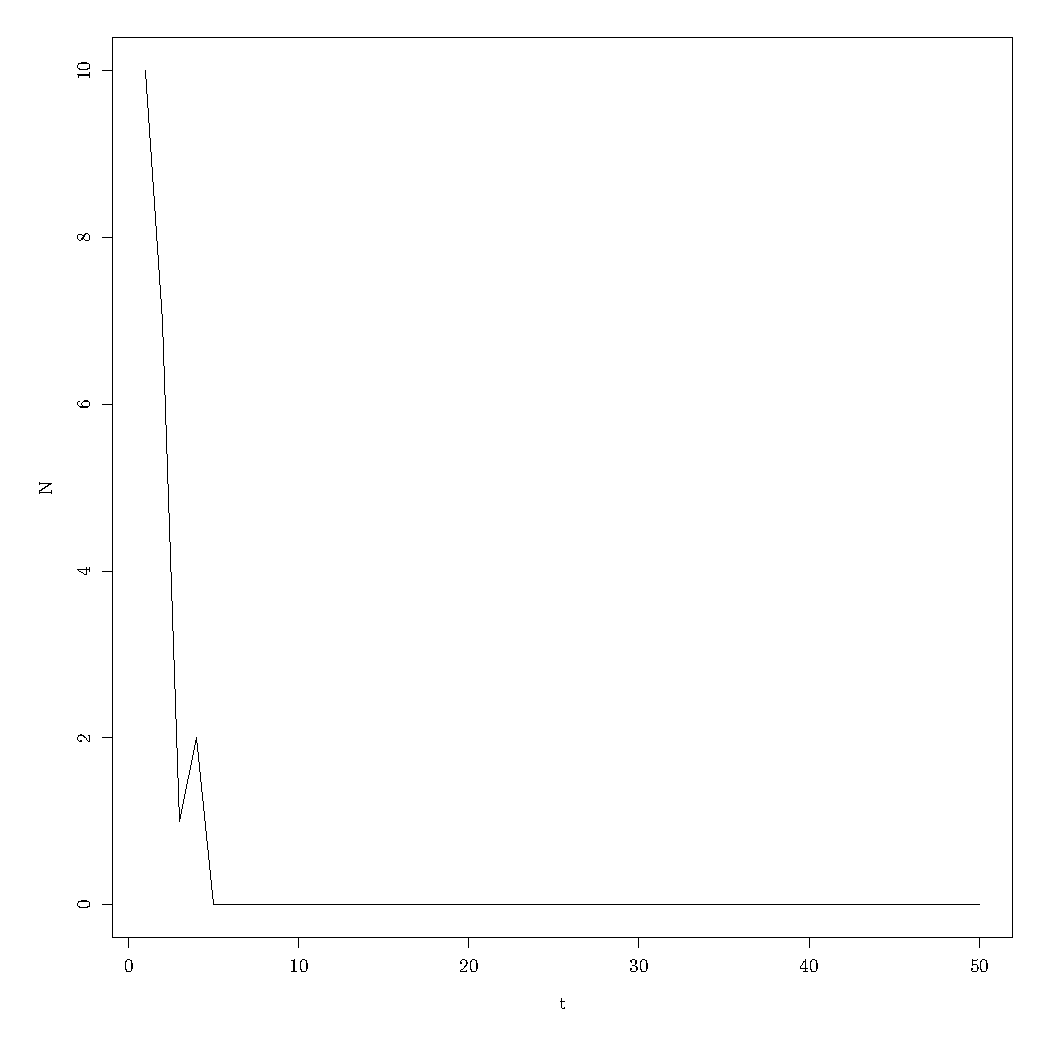
\includegraphics[width=0.5\textwidth]{figure/dice9-1} 

}



\end{knitrout}
Now we repeat the simulation $200$ times and look at the results (the code is not shown, else the previous exercise would become a bit too easy...)
\begin{center}
\begin{tabular}{c c}

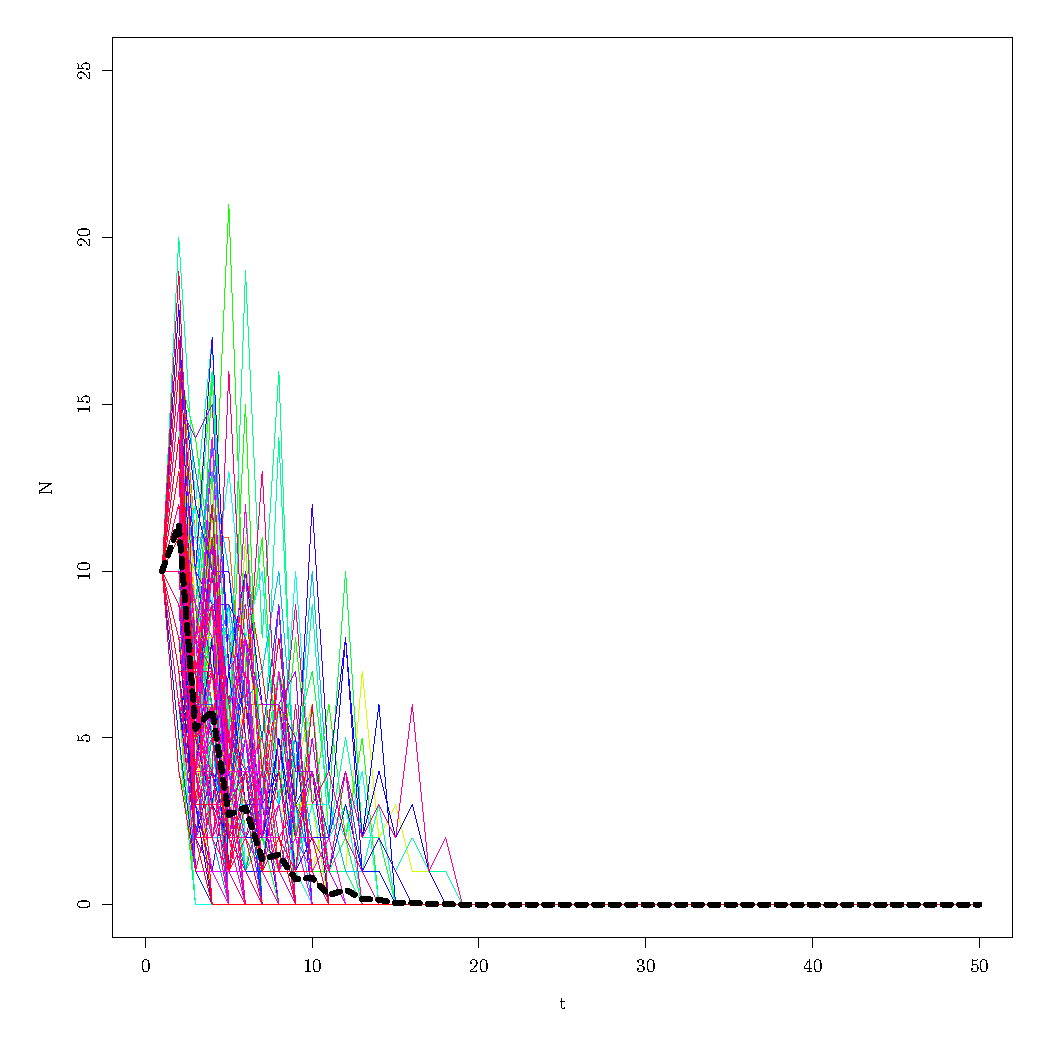
\includegraphics[width=0.5\textwidth]{figure/dice10-1} 
 & 
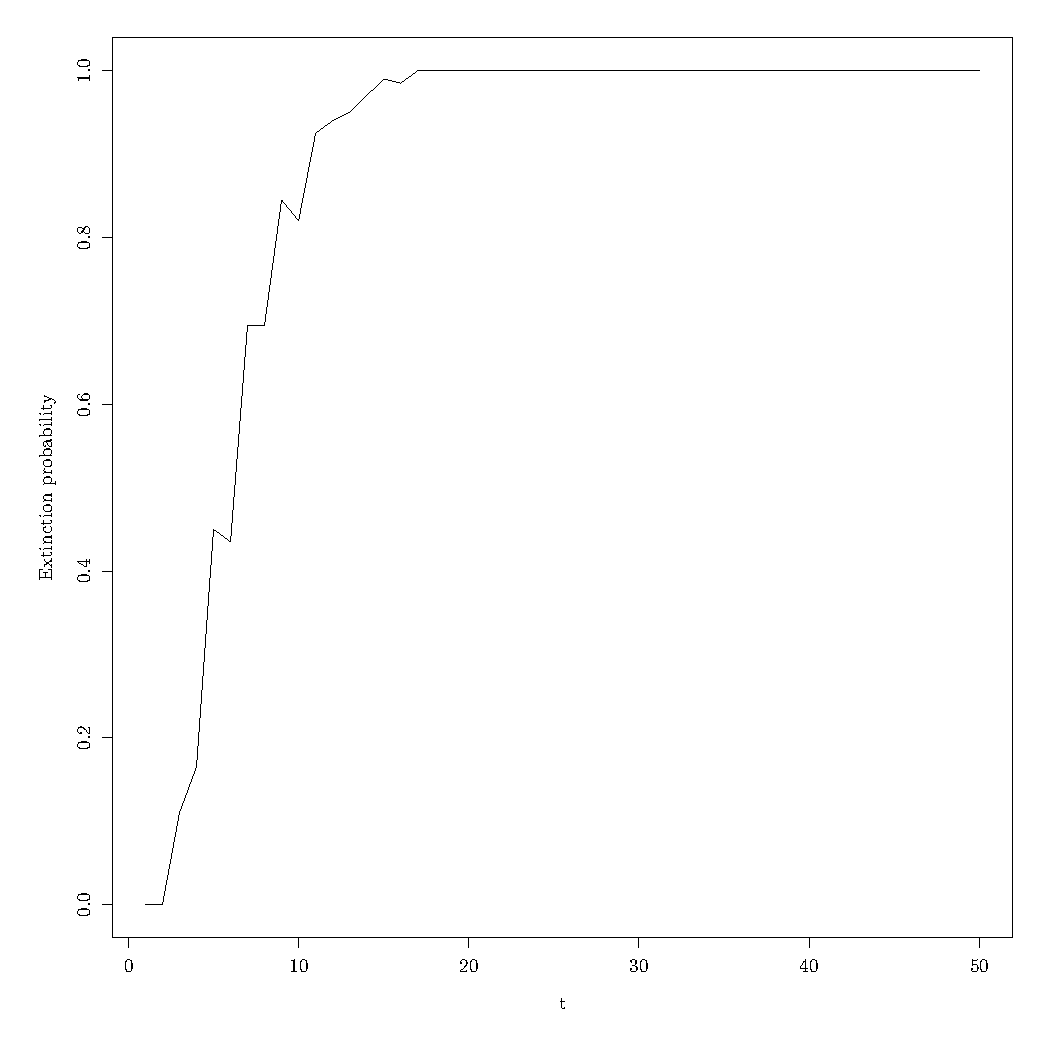
\includegraphics[width=0.5\textwidth]{figure/dice10-2} 

\end{tabular}
\end{center}
Only because we took into account demographic stochasticity, we see that the population goes extinct in $100\%$ of the simulations. If we compare this to the case where we have just $\boldsymbol{A_1}$ and deterministically apply this matrix every time step:
\begin{knitrout}
\definecolor{shadecolor}{rgb}{0.969, 0.969, 0.969}\color{fgcolor}\begin{kframe}
\begin{alltt}
\hlstd{A1}\hlkwb{<-}\hlkwd{matrix}\hlstd{(}\hlkwd{c}\hlstd{(}\hlnum{0}\hlstd{,}\hlnum{0.25}\hlstd{,}\hlnum{2}\hlstd{,}\hlnum{0.5}\hlstd{),} \hlkwc{nr}\hlstd{=}\hlnum{2}\hlstd{)}
\hlstd{timesteps}\hlkwb{<-}\hlnum{50}
\hlstd{N}\hlkwb{<-}\hlkwd{matrix}\hlstd{(}\hlnum{NA}\hlstd{,}\hlkwc{ncol}\hlstd{=timesteps,}\hlkwc{nrow}\hlstd{=}\hlnum{2}\hlstd{)}
\hlstd{N[,}\hlnum{1}\hlstd{]}\hlkwb{<-}\hlkwd{c}\hlstd{(}\hlnum{5}\hlstd{,}\hlnum{5}\hlstd{)}

\hlkwa{for}\hlstd{(t} \hlkwa{in} \hlnum{2}\hlopt{:}\hlstd{timesteps)\{}
   \hlstd{N[,t]}\hlkwb{<-}\hlstd{A1}\hlopt\hlstd{N[,t}\hlopt{-}\hlnum{1}\hlstd{]}
\hlstd{\}}

\hlstd{Ntot}\hlkwb{<-}\hlkwd{colSums}\hlstd{(N)}
\hlkwd{plot}\hlstd{(}\hlnum{1}\hlopt{:}\hlstd{timesteps,Ntot,}\hlkwc{type}\hlstd{=}\hlstr{"l"}\hlstd{,}\hlkwc{xlab}\hlstd{=}\hlstr{"t"}\hlstd{,}\hlkwc{ylab}\hlstd{=}\hlstr{"N"}\hlstd{)}
\end{alltt}
\end{kframe}

{\centering 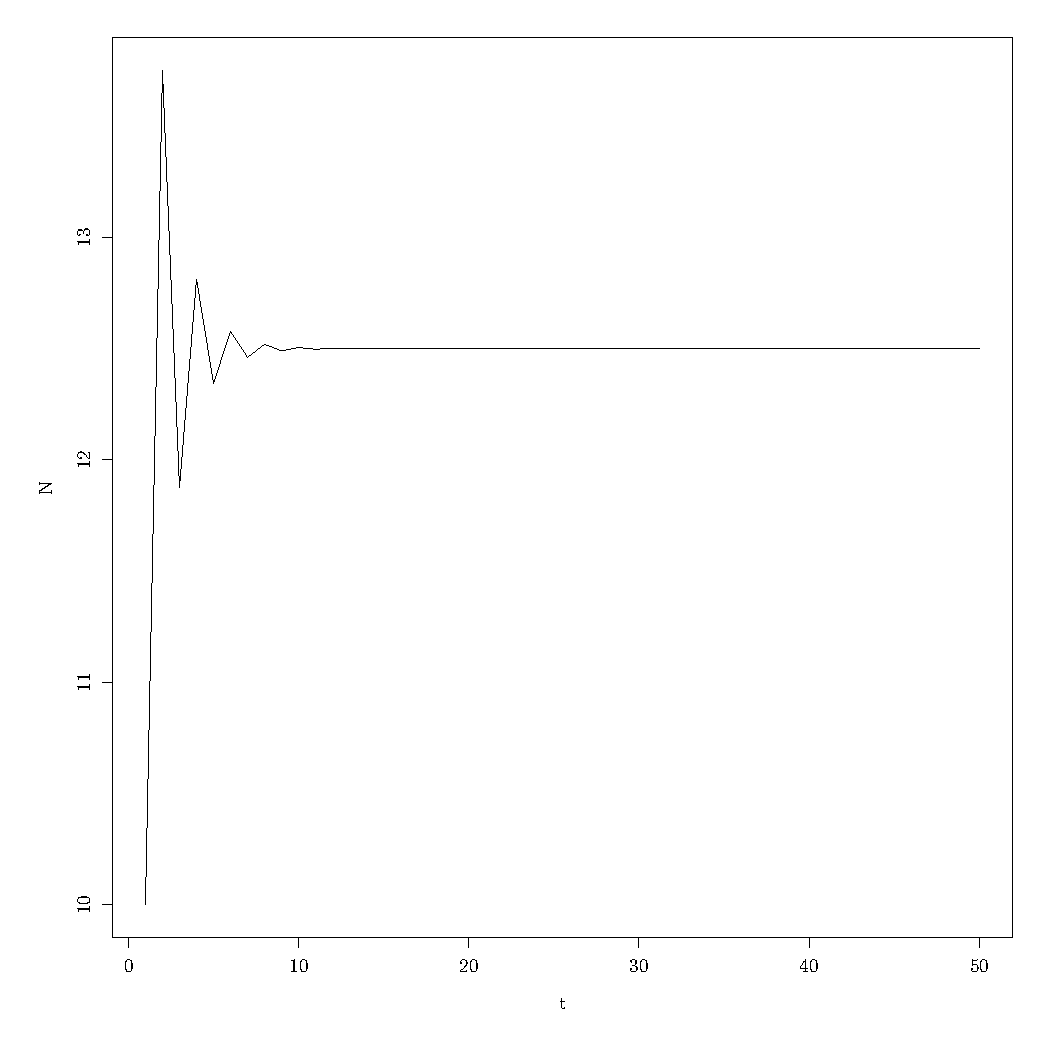
\includegraphics[width=0.5\textwidth]{figure/dice11-1} 

}



\end{knitrout}
We see that here as expected (because $\lambda=1$) the population size stabilizes at one single value ($12.5$). 

\section{Metapopulation dynamics}

So far we have considered only populations in isolation of each other. For instance, in practical 9 we have compared two populations of yellow-necked mice, but have assumed that they were not exchanging migrants. More in general, in all matrix models so far, we have completely ignored the fact that new individuals appear in a population not only because of birth, but also because of immigration. Likewise, death is not the only factor removing individuals from a population, permanent emigration does the job as effectively. 



\begin{figure}
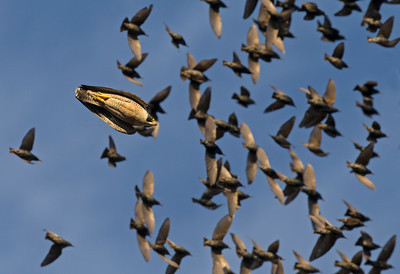
\includegraphics[width=0.95\textwidth]{peregrine}
\caption{\label{fig:peregrine}One of these birds is a peregrine falcon in a dive attack. The other birds are starlings and are in trouble. Populations of peregrine falcons, and other bird species, have declined during the 20th century in North America and Europe as a result of the massive use of the insecticide dichlorodiphenyltrichloroethane. DDT, which causes eggshell thinning, has now been banned from these regions but is still used in tropical regions to fight malaria. Picture by Rob Palmer.}
\end{figure}

Let us consider two populations of peregrine falcons. 
The demography of the two populations is summarized by the Leslie matrices $\boldsymbol{B_1}$ and $\boldsymbol{B_2}$ and by the associated asymptotic growth rates:
\begin{align*}\boldsymbol{B_1} &=% latex table generated in R 3.2.3 by xtable 1.8-0 package
% Mon Mar 14 13:21:49 2016
\begin{pmatrix}{}
  0.00 & 0.25 \\ 
  0.72 & 0.77 \\ 
  \end{pmatrix}
& \boldsymbol{B_2} &=% latex table generated in R 3.2.3 by xtable 1.8-0 package
% Mon Mar 14 13:21:49 2016
\begin{pmatrix}{}
  0.00 & 0.32 \\ 
  0.74 & 0.79 \\ 
  \end{pmatrix}
\\ \lambda &= 0.9579092 &\lambda &= 1.021758\end{align*}
One of the populations seem to be in good shape, while the other one is likely to be declining (but remember that stochasticity can make predictions based on asymptotic behaviour unreliable). Let us assume that the differences between the two populations is due to the massive use of DDT as an insecticide around population 1, while population 2 is located in a remote mountain area with less human influence.

For convenience, we can write these two matrices into a single matrix, $\boldsymbol{B}$, of dimension $4\times 4$:
\begin{align*}\boldsymbol{B} &=% latex table generated in R 3.2.3 by xtable 1.8-0 package
% Mon Mar 14 13:21:49 2016
\begin{pmatrix}{}
  0.00 & 0.25 & 0.00 & 0.00 \\ 
  0.72 & 0.77 & 0.00 & 0.00 \\ 
  0.00 & 0.00 & 0.00 & 0.32 \\ 
  0.00 & 0.00 & 0.74 & 0.79 \\ 
  \end{pmatrix}
\end{align*}

These two populations are not ecologically isolated, however, and they exchange a number of migrants, both juveniles and adults every year. 
Migration rates vary depending on age, and are not symmetrical. Thus, $73\%$ of juveniles born in the population 1 stay there (and therefor $50\%$ emigrate to population 2), while $50\%$ of juveniles born in population 2 stay there ($50\%$ emmigrate). 
These rates are summarized in the matrix $\boldsymbol{M_j}$:
\begin{align*}\boldsymbol{M_j} &=% latex table generated in R 3.2.3 by xtable 1.8-0 package
% Mon Mar 14 13:21:49 2016
\begin{pmatrix}{}
  0.73 & 0.50 \\ 
  0.27 & 0.50 \\ 
  \end{pmatrix}
\end{align*}
Similarly, migration rates for adults are summarized in matrix $\boldsymbol{M_a}$:
\begin{align*}\boldsymbol{M_a} &=% latex table generated in R 3.2.3 by xtable 1.8-0 package
% Mon Mar 14 13:21:49 2016
\begin{pmatrix}{}
  0.50 & 0.20 \\ 
  0.50 & 0.80 \\ 
  \end{pmatrix}
\end{align*}

We also define a matrix $\boldsymbol{M}$ summarizing the migration rates:
\begin{align*}\boldsymbol{M} &=% latex table generated in R 3.2.3 by xtable 1.8-0 package
% Mon Mar 14 13:21:49 2016
\begin{pmatrix}{}
  0.73 & 0.50 & 0.00 & 0.00 \\ 
  0.27 & 0.50 & 0.00 & 0.00 \\ 
  0.00 & 0.00 & 0.50 & 0.20 \\ 
  0.00 & 0.00 & 0.50 & 0.80 \\ 
  \end{pmatrix}
\end{align*}


What is the proportion of adults migrating from population 2 to population 1? (dumb question, just to check)\\

We would like to modify the matrix $\boldsymbol{B}$ so that it contains the migration rates. \\
What are the two assumptions you have to make before you can start? 
(hints: one is about population size, and one about timing)\\% even ratio of population sizes + timing of reproduction VS. migration


This task is not absolutely trivial to do mathematically because $\boldsymbol{M}$ is organized by age, while $\boldsymbol{B}$ is organized by site. 
Nevertheless, by thinking carefully, you can find what should be the elements of the matrix one by one. We just need to understand how the matrix is organized.
You can visualize four compartments in \boldsymbol{A}:
\begin{align*}
\boldsymbol{A}=
\begin{pmatrix}
\boldsymbol{\color{red}{A_1}} & \boldsymbol{\color{orange}{A_2}} \\
\boldsymbol{\color{blue}{A_3}} & \boldsymbol{\color{purple}{A_4}}
\end{pmatrix}
=\begin{pmatrix}
  \color{red}{a_{11}} & \color{red}{a_{12}} & \color{orange}{a_{13}} & \color{orange}{a_{14}}\\
  \color{red}{a_{21}} & \color{red}{a_{22}} & \color{orange}{a_{23}} & \color{orange}{a_{24}}\\
  \color{blue}{a_{31}} & \color{blue}{a_{32}} & \color{purple}{a_{33}} & \color{purple}{a_{34}}\\
  \color{blue}{a_{41}} & \color{blue}{a_{42}} & \color{purple}{a_{43}} & \color{purple}{a_{44}}\\
\end{pmatrix}
\end{align*}
In {\color{red}{red}}, the sub-matrix $\boldsymbol{\color{red}{A_1}}$ contains the contribution of the population $1$ to itself, that is, the fertility ($f_1$) and survival ($\phi_{j1}$ & $\phi_{a1}$) rates, corrected for emigration out of $1$ ($d_1$). Within $\boldsymbol{\color{red}{A_1}}$, $\color{red}{a_{11}}$ is the contribution of the juvenile age class to itself, within population $1$. Clearly this is zero, for juveniles do not reproduce. $\color{red}{a_{21}}$ is the contribution of juveniles to adults, within population $1$, and is the product of juvenile survival by the proportion of non-migrating adults (not the proportion of non-migrating juveniles, because of the order of sequence of life-history events we assume). 
What are $\color{red}{a_{12}}$ and $\color{red}{a_{22}}$?\\

Let's now look at the rest of our matrix $\boldsymbol{A}$. The sub-matrix $\boldsymbol{\color{orange}{A_2}}$ represents the contributions of the population $2$ to the population $1$, that is, the fertility ($f_2$) and survival ($\phi_{j2}$ & $\phi_{a2}$) rates within population $2$, multiplied by the rate of emigration out of $2$ ($d_2$).

You should now be able to guess the rest and write $\boldsymbol{A}$ completely, using symbols $f$ (fertility), $\phi$ (survival) and $d$ (emigration), and indexes $1$ (population $1$), $2$ (population $2$), $j$ (juvenile) and $a$ (adult).
Do it, and the proceed to the numerical application.\\


During the lectures, you have seen how one can use matrix algebra, instead of biological thinking (as you just did), to efficiently obtain this meta-population matrix $\boldsymbol{A}$, using a vec-permutation matrix, \boldsymbol{P}.

\boldsymbol{P} can be defined as:
\begin{align*}
\boldsymbol{P} = \sum\limits_{i=1}^s  \sum\limits_{j=1}^p \boldsymbol{E_{ij}} \bigotimes \boldsymbol{E_{ij}}^T\text{, }
\end{align*}
where $s$ and $p$ are the dimensions of the two square matrices to be combined, $\bigotimes$ is the Kronecker product (google it if you don't know it, it's nothing difficult) and where $\boldsymbol{E_{ij}}$ is a matrix of dimension $s\times p$ containing a $1$ on the $i^{th}$ line of the $j^{th}$ column, and $0$ elsewhere. 
For instance, for $s=p=2$, $\boldsymbol{E_{1,2}} = \begin{pmatrix} 0 & 1 \\ 0 & 0 \end{pmatrix}$.
Can you write a code that calculates \boldsymbol{P}?



From the lecture, you know that
\begin{align*}
\boldsymbol{A} = \boldsymbol{P^T}\boldsymbol{M}\boldsymbol{P}\boldsymbol{B} \text{,}
\end{align*}
where $\boldsymbol{P^T}$ is the transposition of \boldsymbol{P}. 
Write a code that computes $\boldsymbol{A}$. You will need to know how to multiply matrices in \texttt{R}, and you might want to know how to transpose matrices (although here it is useless because $\boldsymbol{P^T}=\boldsymbol{P}$).


\begin{knitrout}
\definecolor{shadecolor}{rgb}{0.969, 0.969, 0.969}\color{fgcolor}\begin{kframe}
\begin{alltt}
\hlcom{# Create M, the block diagonal matrix of movement matrices}

\hlstd{A1} \hlcom{#check what it looks like}
\end{alltt}
\begin{verbatim}
##      [,1] [,2]
## [1,] 0.00  2.0
## [2,] 0.25  0.5
\end{verbatim}
\begin{alltt}
\hlkwd{eigen.analysis}\hlstd{(A1)} \hlcom{# Check local and metapoulation growth rates an have a look at the sensitivity matrix}
\end{alltt}
\begin{verbatim}
## $lambda1
## [1] 1
## 
## $stable.stage
## [1] 0.6666667 0.3333333
## 
## $sensitivities
##          [,1]      [,2]
## [1,] 0.000000 0.1666667
## [2,] 1.333333 0.6666667
## 
## $elasticities
##           [,1]      [,2]
## [1,] 0.0000000 0.3333333
## [2,] 0.3333333 0.3333333
## 
## $repro.value
## [1] 1 4
## 
## $damping.ratio
## [1] 2
\end{verbatim}
\begin{alltt}
\hlstd{lambda} \hlkwb{<-} \hlkwd{eigen.analysis}\hlstd{(A)}\hlopt{$}\hlstd{lambda1} \hlcom{# how does the metapoulation growth rate compare to local growth rates?}


\hlcom{## Sensitivity & elasticity of metapopulation growth rate to demography and dispersal}

\hlstd{Asens1}\hlkwb{<-}\hlkwd{eigen.analysis}\hlstd{(A1)}\hlopt{$}\hlstd{sensitivities} \hlcom{# the A sensitivity matrix}
\hlstd{Asens2}\hlkwb{<-}\hlkwd{eigen.analysis}\hlstd{(A2)}\hlopt{$}\hlstd{sensitivities} \hlcom{# the A sensitivity matrix}
\end{alltt}


{\ttfamily\noindent\bfseries\color{errorcolor}{\#\# Error in as.matrix(x): object 'A2' not found}}\begin{alltt}
\hlstd{Asens3}\hlkwb{<-}\hlkwd{eigen.analysis}\hlstd{(A3)}\hlopt{$}\hlstd{sensitivities} \hlcom{# the A sensitivity matrix}
\end{alltt}


{\ttfamily\noindent\bfseries\color{errorcolor}{\#\# Error in as.matrix(x): object 'A3' not found}}\begin{alltt}
\hlstd{Asens4}\hlkwb{<-}\hlkwd{eigen.analysis}\hlstd{(A4)}\hlopt{$}\hlstd{sensitivities} \hlcom{# the A sensitivity matrix}
\end{alltt}


{\ttfamily\noindent\bfseries\color{errorcolor}{\#\# Error in as.matrix(x): object 'A4' not found}}\begin{alltt}
\hlstd{Bsens1}\hlkwb{<-}\hlkwd{t}\hlstd{(P)} \hlopt \hlkwd{t}\hlstd{(M)} \hlopt \hlstd{P} \hlopt \hlstd{Asens1} \hlcom{# demography sensitivities}
\end{alltt}


{\ttfamily\noindent\bfseries\color{errorcolor}{\#\# Error in t(P) \%*\% t(M) \%*\% P \%*\% Asens1: non-conformable arguments}}\begin{alltt}
\hlstd{Bsens2}\hlkwb{<-}\hlstd{Asens2} \hlopt \hlkwd{t}\hlstd{(P)} \hlopt \hlkwd{t}\hlstd{(M)} \hlopt \hlstd{P} \hlcom{# demography sensitivities}
\end{alltt}


{\ttfamily\noindent\bfseries\color{errorcolor}{\#\# Error in eval(expr, envir, enclos): object 'Asens2' not found}}\begin{alltt}
\hlstd{Bsens3}\hlkwb{<-}\hlkwd{t}\hlstd{(P)} \hlopt \hlkwd{t}\hlstd{(M)} \hlopt \hlstd{Asens3} \hlopt \hlstd{P} \hlcom{# demography sensitivities}
\end{alltt}


{\ttfamily\noindent\bfseries\color{errorcolor}{\#\# Error in eval(expr, envir, enclos): object 'Asens3' not found}}\begin{alltt}
\hlstd{Bsens4}\hlkwb{<-}\hlkwd{t}\hlstd{(P)} \hlopt \hlstd{Asens4} \hlopt \hlkwd{t}\hlstd{(M)} \hlopt \hlstd{P} \hlcom{# demography sensitivities}
\end{alltt}


{\ttfamily\noindent\bfseries\color{errorcolor}{\#\# Error in eval(expr, envir, enclos): object 'Asens4' not found}}\begin{alltt}
\hlstd{Belas}\hlkwb{<-}\hlstd{B} \hlopt{*} \hlstd{Bsens} \hlopt{/} \hlstd{lambda}  \hlcom{# demography elasticities}
\end{alltt}


{\ttfamily\noindent\bfseries\color{errorcolor}{\#\# Error in eval(expr, envir, enclos): object 'Bsens' not found}}\begin{alltt}
\hlkwd{sum}\hlstd{(Belas[}\hlnum{1}\hlopt{:}\hlnum{2}\hlstd{,}\hlnum{1}\hlopt{:}\hlnum{2}\hlstd{])} \hlcom{# contribution from patch 1 to metapopulation growth rate }
\end{alltt}


{\ttfamily\noindent\bfseries\color{errorcolor}{\#\# Error in eval(expr, envir, enclos): object 'Belas' not found}}\begin{alltt}
\hlkwd{sum}\hlstd{(Belas[}\hlnum{3}\hlopt{:}\hlnum{4}\hlstd{,}\hlnum{3}\hlopt{:}\hlnum{4}\hlstd{])} \hlcom{# contribution from patch 2 to metapopulation growth rate }
\end{alltt}


{\ttfamily\noindent\bfseries\color{errorcolor}{\#\# Error in eval(expr, envir, enclos): object 'Belas' not found}}\begin{alltt}
\hlstd{Msens}\hlkwb{=}\hlstd{P} \hlopt \hlkwd{t}\hlstd{(B)} \hlopt \hlstd{Asens} \hlopt \hlkwd{t}\hlstd{(P)} \hlcom{# movement sensitivities}
\end{alltt}


{\ttfamily\noindent\bfseries\color{errorcolor}{\#\# Error in eval(expr, envir, enclos): object 'Asens' not found}}\begin{alltt}
\hlcom{# You'll realize that interpreting Movement sensitivities is rather difficult. A better approach would be to estimate the lower-level sensitivities for the dispersal rate, d (see H&C 2005)}

\hlopt{-}\hlnum{1} \hlopt{*} \hlstd{Msens[}\hlnum{1}\hlstd{,}\hlnum{1}\hlstd{]} \hlopt{+} \hlnum{1} \hlopt{*} \hlstd{Msens[}\hlnum{1}\hlstd{,}\hlnum{2}\hlstd{]} \hlopt{+} \hlnum{1} \hlopt{*} \hlstd{Msens[}\hlnum{2}\hlstd{,}\hlnum{1}\hlstd{]} \hlopt{-} \hlnum{1} \hlopt{*} \hlstd{Msens[}\hlnum{2}\hlstd{,}\hlnum{2}\hlstd{]}
\end{alltt}


{\ttfamily\noindent\bfseries\color{errorcolor}{\#\# Error in eval(expr, envir, enclos): object 'Msens' not found}}\begin{alltt}
\hlcom{###############################################################}


\hlcom{# Gull example (Lebreton, 1966)}

\hlkwd{rm}\hlstd{(}\hlkwc{list}\hlstd{=}\hlkwd{ls}\hlstd{(}\hlkwc{all}\hlstd{=}\hlnum{TRUE}\hlstd{))}

\hlstd{B1}\hlkwb{<-}\hlkwd{matrix}\hlstd{(}\hlkwd{c}\hlstd{(}\hlnum{0}\hlstd{,}\hlnum{0.096}\hlstd{,}\hlnum{0.160}\hlstd{,}\hlnum{0.224}\hlstd{,}\hlnum{0.320}\hlstd{,}\hlnum{0.80}\hlstd{,}\hlnum{0}\hlstd{,}\hlnum{0}\hlstd{,}\hlnum{0}\hlstd{,}\hlnum{0}\hlstd{,}\hlnum{0}\hlstd{,}\hlnum{0.82}\hlstd{,}\hlnum{0}\hlstd{,}\hlnum{0}\hlstd{,}\hlnum{0}\hlstd{,}\hlnum{0}\hlstd{,}\hlnum{0}\hlstd{,}\hlnum{0.82}\hlstd{,}\hlnum{0}\hlstd{,}\hlnum{0}\hlstd{,}\hlnum{0}\hlstd{,}\hlnum{0}\hlstd{,}\hlnum{0}\hlstd{,}\hlnum{0.82}\hlstd{,}\hlnum{0.82}\hlstd{),}\hlnum{5}\hlstd{,}\hlnum{5}\hlstd{,}\hlkwc{byrow}\hlstd{=T)}    \hlcom{# for patch 1}

\hlstd{B2}\hlkwb{<-}\hlkwd{matrix}\hlstd{(}\hlkwd{c}\hlstd{(}\hlnum{0}\hlstd{,}\hlnum{0.1}\hlstd{,}\hlnum{0.160}\hlstd{,}\hlnum{0.20}\hlstd{,}\hlnum{0.20}\hlstd{,}\hlnum{0.80}\hlstd{,}\hlnum{0}\hlstd{,}\hlnum{0}\hlstd{,}\hlnum{0}\hlstd{,}\hlnum{0}\hlstd{,}\hlnum{0}\hlstd{,}\hlnum{0.82}\hlstd{,}\hlnum{0}\hlstd{,}\hlnum{0}\hlstd{,}\hlnum{0}\hlstd{,}\hlnum{0}\hlstd{,}\hlnum{0}\hlstd{,}\hlnum{0.82}\hlstd{,}\hlnum{0}\hlstd{,}\hlnum{0}\hlstd{,}\hlnum{0}\hlstd{,}\hlnum{0}\hlstd{,}\hlnum{0}\hlstd{,}\hlnum{0.82}\hlstd{,}\hlnum{0.82}\hlstd{),}\hlnum{5}\hlstd{,}\hlnum{5}\hlstd{,}\hlkwc{byrow}\hlstd{=T)} \hlcom{# for patch 2}

\hlstd{M1}\hlkwb{<-}\hlkwd{matrix}\hlstd{(}\hlkwd{c}\hlstd{(}\hlnum{0.75}\hlstd{,}\hlnum{0.375}\hlstd{,}\hlnum{0.25}\hlstd{,}\hlnum{0.625}\hlstd{),}\hlnum{2}\hlstd{,}\hlnum{2}\hlstd{,}\hlkwc{byrow}\hlstd{=T)}  \hlcom{# for the first age class}

\hlstd{M5}\hlkwb{<-}\hlstd{M4}\hlkwb{<-}\hlstd{M3}\hlkwb{<-}\hlstd{M2}\hlkwb{<-}\hlkwd{matrix}\hlstd{(}\hlkwd{c}\hlstd{(}\hlnum{1}\hlstd{,}\hlnum{0}\hlstd{,}\hlnum{0}\hlstd{,}\hlnum{1}\hlstd{),}\hlnum{2}\hlstd{,}\hlnum{2}\hlstd{,}\hlkwc{byrow}\hlstd{=T)} \hlcom{# for the rest}


\hlcom{# This time, dispersal takes place before demography, and assume that population vector is arranged by stages}

\hlcom{# Using a similar approach to the Gull example above, try to estimate the relative contribution of each patch to the metapopulation growth rate (demographic elasticities).}
\end{alltt}
\end{kframe}
\end{knitrout}

\begin{knitrout}
\definecolor{shadecolor}{rgb}{0.969, 0.969, 0.969}\color{fgcolor}\begin{kframe}
\begin{alltt}
\hlcom{#############################################}

\hlstd{s}\hlkwb{=}\hlkwd{nrow}\hlstd{(B1)} \hlcom{# number of stages}

\hlstd{p}\hlkwb{=}\hlkwd{nrow}\hlstd{(M1)} \hlcom{# number of patches}


\hlcom{# Create the block diagonal matrix of demographic projection matrices}

\hlstd{B}\hlkwb{<-}\hlkwd{matrix}\hlstd{(}\hlnum{0}\hlstd{,p}\hlopt{*}\hlstd{s,p}\hlopt{*}\hlstd{s)}

\hlstd{B[}\hlnum{1}\hlopt{:}\hlnum{5}\hlstd{,}\hlnum{1}\hlopt{:}\hlnum{5}\hlstd{]}\hlkwb{<-}\hlstd{B1}

\hlstd{B[}\hlnum{6}\hlopt{:}\hlnum{10}\hlstd{,}\hlnum{6}\hlopt{:}\hlnum{10}\hlstd{]}\hlkwb{<-}\hlstd{B2}

\hlstd{B} \hlcom{#check}
\end{alltt}
\begin{verbatim}
##       [,1]  [,2] [,3]  [,4] [,5] [,6] [,7] [,8] [,9] [,10]
##  [1,]  0.0 0.096 0.16 0.224 0.32  0.0 0.00 0.00 0.00  0.00
##  [2,]  0.8 0.000 0.00 0.000 0.00  0.0 0.00 0.00 0.00  0.00
##  [3,]  0.0 0.820 0.00 0.000 0.00  0.0 0.00 0.00 0.00  0.00
##  [4,]  0.0 0.000 0.82 0.000 0.00  0.0 0.00 0.00 0.00  0.00
##  [5,]  0.0 0.000 0.00 0.820 0.82  0.0 0.00 0.00 0.00  0.00
##  [6,]  0.0 0.000 0.00 0.000 0.00  0.0 0.10 0.16 0.20  0.20
##  [7,]  0.0 0.000 0.00 0.000 0.00  0.8 0.00 0.00 0.00  0.00
##  [8,]  0.0 0.000 0.00 0.000 0.00  0.0 0.82 0.00 0.00  0.00
##  [9,]  0.0 0.000 0.00 0.000 0.00  0.0 0.00 0.82 0.00  0.00
## [10,]  0.0 0.000 0.00 0.000 0.00  0.0 0.00 0.00 0.82  0.82
\end{verbatim}
\begin{alltt}
\hlcom{# Create M, the block diagonal matrix of movement matrices}

\hlstd{M}\hlkwb{=}\hlkwd{matrix}\hlstd{(}\hlnum{0}\hlstd{,p}\hlopt{*}\hlstd{s,p}\hlopt{*}\hlstd{s)}

\hlstd{M[}\hlnum{1}\hlopt{:}\hlnum{2}\hlstd{,}\hlnum{1}\hlopt{:}\hlnum{2}\hlstd{]}\hlkwb{<-}\hlstd{M1}

\hlstd{M[}\hlnum{3}\hlopt{:}\hlnum{4}\hlstd{,}\hlnum{3}\hlopt{:}\hlnum{4}\hlstd{]}\hlkwb{<-}\hlstd{M2}
\hlstd{M[}\hlnum{5}\hlopt{:}\hlnum{6}\hlstd{,}\hlnum{5}\hlopt{:}\hlnum{6}\hlstd{]}\hlkwb{<-}\hlstd{M3}
\hlstd{M[}\hlnum{7}\hlopt{:}\hlnum{8}\hlstd{,}\hlnum{7}\hlopt{:}\hlnum{8}\hlstd{]}\hlkwb{<-}\hlstd{M4}
\hlstd{M[}\hlnum{9}\hlopt{:}\hlnum{10}\hlstd{,}\hlnum{9}\hlopt{:}\hlnum{10}\hlstd{]}\hlkwb{<-}\hlstd{M5}

\hlstd{M} \hlcom{#check}
\end{alltt}
\begin{verbatim}
##       [,1]  [,2] [,3] [,4] [,5] [,6] [,7] [,8] [,9] [,10]
##  [1,] 0.75 0.375    0    0    0    0    0    0    0     0
##  [2,] 0.25 0.625    0    0    0    0    0    0    0     0
##  [3,] 0.00 0.000    1    0    0    0    0    0    0     0
##  [4,] 0.00 0.000    0    1    0    0    0    0    0     0
##  [5,] 0.00 0.000    0    0    1    0    0    0    0     0
##  [6,] 0.00 0.000    0    0    0    1    0    0    0     0
##  [7,] 0.00 0.000    0    0    0    0    1    0    0     0
##  [8,] 0.00 0.000    0    0    0    0    0    1    0     0
##  [9,] 0.00 0.000    0    0    0    0    0    0    1     0
## [10,] 0.00 0.000    0    0    0    0    0    0    0     1
\end{verbatim}
\begin{alltt}
\hlcom{# create P, the vec-permutation matrix}

\hlstd{P}\hlkwb{<-}\hlkwd{matrix}\hlstd{(}\hlnum{0}\hlstd{,s}\hlopt{*}\hlstd{p,s}\hlopt{*}\hlstd{p)}
\hlkwa{for} \hlstd{(i} \hlkwa{in} \hlnum{1}\hlopt{:}\hlstd{s)\{}
        \hlkwa{for} \hlstd{(j} \hlkwa{in} \hlnum{1}\hlopt{:}\hlstd{p)\{}
                \hlstd{E}\hlkwb{=}\hlkwd{matrix}\hlstd{(}\hlnum{0}\hlstd{,s,p)}
        \hlstd{E[i,j]}\hlkwb{<-}\hlnum{1}
        \hlstd{P}\hlkwb{<-}\hlstd{P}\hlopt{+}\hlstd{E}\hlopt\hlkwd{t}\hlstd{(E)} \hlcom{# %x% is the Kronecker product}
        \hlstd{\}\}}


\hlcom{# create the Metapopulation Projection Matrix, A}

\hlstd{A}\hlkwb{<-} \hlstd{P} \hlopt \hlstd{B} \hlopt \hlkwd{t}\hlstd{(P)} \hlopt \hlstd{M}
\hlstd{A} \hlcom{#check what it looks like}
\end{alltt}
\begin{verbatim}
##       [,1] [,2]  [,3] [,4] [,5] [,6]  [,7] [,8] [,9] [,10]
##  [1,]  0.0  0.0 0.096 0.00 0.16 0.00 0.224 0.00 0.32  0.00
##  [2,]  0.0  0.0 0.000 0.10 0.00 0.16 0.000 0.20 0.00  0.20
##  [3,]  0.6  0.3 0.000 0.00 0.00 0.00 0.000 0.00 0.00  0.00
##  [4,]  0.2  0.5 0.000 0.00 0.00 0.00 0.000 0.00 0.00  0.00
##  [5,]  0.0  0.0 0.820 0.00 0.00 0.00 0.000 0.00 0.00  0.00
##  [6,]  0.0  0.0 0.000 0.82 0.00 0.00 0.000 0.00 0.00  0.00
##  [7,]  0.0  0.0 0.000 0.00 0.82 0.00 0.000 0.00 0.00  0.00
##  [8,]  0.0  0.0 0.000 0.00 0.00 0.82 0.000 0.00 0.00  0.00
##  [9,]  0.0  0.0 0.000 0.00 0.00 0.00 0.820 0.00 0.82  0.00
## [10,]  0.0  0.0 0.000 0.00 0.00 0.00 0.000 0.82 0.00  0.82
\end{verbatim}
\begin{alltt}
\hlkwd{eigen.analysis}\hlstd{(A)} \hlcom{# Check local and metapoulation growth rates an have a look at the sensitivity matrix}
\end{alltt}
\begin{verbatim}
## $lambda1
## [1] 0.9970859
## 
## $stable.stage
##  [1] 0.12952855 0.05171024 0.09350268 0.05191211 0.07689628
##  [6] 0.04269234 0.06323924 0.03511004 0.29283071 0.16257780
## 
## $sensitivities
##             [,1]       [,2]       [,3]       [,4]
##  [1,] 0.00000000 0.00000000 0.07042373 0.00000000
##  [2,] 0.00000000 0.00000000 0.00000000 0.03256113
##  [3,] 0.13514559 0.05395267 0.00000000 0.00000000
##  [4,] 0.08092901 0.03230839 0.00000000 0.00000000
##  [5,] 0.00000000 0.00000000 0.11038107 0.00000000
##  [6,] 0.00000000 0.00000000 0.00000000 0.03546815
##  [7,] 0.00000000 0.00000000 0.00000000 0.00000000
##  [8,] 0.00000000 0.00000000 0.00000000 0.00000000
##  [9,] 0.00000000 0.00000000 0.00000000 0.00000000
## [10,] 0.00000000 0.00000000 0.00000000 0.00000000
##             [,5]       [,6]       [,7]       [,8]      [,9]
##  [1,] 0.05791623 0.00000000 0.04763011 0.00000000 0.2205523
##  [2,] 0.00000000 0.02677817 0.00000000 0.02202227 0.0000000
##  [3,] 0.00000000 0.00000000 0.00000000 0.00000000 0.0000000
##  [4,] 0.00000000 0.00000000 0.00000000 0.00000000 0.0000000
##  [5,] 0.00000000 0.00000000 0.00000000 0.00000000 0.0000000
##  [6,] 0.00000000 0.00000000 0.00000000 0.00000000 0.0000000
##  [7,] 0.09908034 0.00000000 0.00000000 0.00000000 0.0000000
##  [8,] 0.00000000 0.03024314 0.00000000 0.00000000 0.0000000
##  [9,] 0.00000000 0.00000000 0.08606919 0.00000000 0.3985453
## [10,] 0.00000000 0.00000000 0.00000000 0.02487186 0.0000000
##           [,10]
##  [1,] 0.0000000
##  [2,] 0.1019746
##  [3,] 0.0000000
##  [4,] 0.0000000
##  [5,] 0.0000000
##  [6,] 0.0000000
##  [7,] 0.0000000
##  [8,] 0.0000000
##  [9,] 0.0000000
## [10,] 0.1151697
## 
## $elasticities
##             [,1]       [,2]        [,3]       [,4]
##  [1,] 0.00000000 0.00000000 0.006780437 0.00000000
##  [2,] 0.00000000 0.00000000 0.000000000 0.00326563
##  [3,] 0.08132434 0.01623311 0.000000000 0.00000000
##  [4,] 0.01623311 0.01620141 0.000000000 0.00000000
##  [5,] 0.00000000 0.00000000 0.090777014 0.00000000
##  [6,] 0.00000000 0.00000000 0.000000000 0.02916889
##  [7,] 0.00000000 0.00000000 0.000000000 0.00000000
##  [8,] 0.00000000 0.00000000 0.000000000 0.00000000
##  [9,] 0.00000000 0.00000000 0.000000000 0.00000000
## [10,] 0.00000000 0.00000000 0.000000000 0.00000000
##             [,5]        [,6]       [,7]        [,8]
##  [1,] 0.00929368 0.000000000 0.01070033 0.000000000
##  [2,] 0.00000000 0.004297029 0.00000000 0.004417327
##  [3,] 0.00000000 0.000000000 0.00000000 0.000000000
##  [4,] 0.00000000 0.000000000 0.00000000 0.000000000
##  [5,] 0.00000000 0.000000000 0.00000000 0.000000000
##  [6,] 0.00000000 0.000000000 0.00000000 0.000000000
##  [7,] 0.08148333 0.000000000 0.00000000 0.000000000
##  [8,] 0.00000000 0.024871858 0.00000000 0.000000000
##  [9,] 0.00000000 0.000000000 0.07078301 0.000000000
## [10,] 0.00000000 0.000000000 0.00000000 0.020454531
##             [,9]      [,10]
##  [1,] 0.07078301 0.00000000
##  [2,] 0.00000000 0.02045453
##  [3,] 0.00000000 0.00000000
##  [4,] 0.00000000 0.00000000
##  [5,] 0.00000000 0.00000000
##  [6,] 0.00000000 0.00000000
##  [7,] 0.00000000 0.00000000
##  [8,] 0.00000000 0.00000000
##  [9,] 0.32776228 0.00000000
## [10,] 0.00000000 0.09471516
## 
## $repro.value
##  [1] 1.0000000 0.8327907 1.3852923 0.8295523 1.5673846
##  [6] 0.9071412 1.7107525 0.9405502 1.8070331 0.9405502
## 
## $damping.ratio
## [1] 1.117914
\end{verbatim}
\begin{alltt}
\hlstd{lambda} \hlkwb{<-} \hlkwd{eigen.analysis}\hlstd{(A)}\hlopt{$}\hlstd{lambda1}

\hlcom{## A sensitivity & elasticity}

\hlstd{analysis}\hlkwb{<-}\hlkwd{eigen.analysis}\hlstd{(A)}

\hlstd{Asens}\hlkwb{<-}\hlstd{analysis}\hlopt{$}\hlstd{sensitivities} \hlcom{# the A sensitivity matrix}

\hlstd{Bsens}\hlkwb{<-}\hlkwd{t}\hlstd{(P)} \hlopt \hlstd{Asens} \hlopt \hlkwd{t}\hlstd{(M)} \hlopt \hlstd{P}    \hlcom{# demography sensitivities}

\hlstd{Belas}\hlkwb{<-}\hlstd{B} \hlopt{*} \hlstd{Bsens} \hlopt{/} \hlstd{lambda}  \hlcom{# demography elasticities}

\hlkwd{sum}\hlstd{(Belas[}\hlnum{1}\hlopt{:}\hlnum{5}\hlstd{,}\hlnum{1}\hlopt{:}\hlnum{5}\hlstd{])}   \hlcom{# contribution from patch 1 to metapopulation growth rate }
\end{alltt}
\begin{verbatim}
## [1] 0.7659205
\end{verbatim}
\begin{alltt}
\hlkwd{sum}\hlstd{(Belas[}\hlnum{6}\hlopt{:}\hlnum{10}\hlstd{,}\hlnum{6}\hlopt{:}\hlnum{10}\hlstd{])} \hlcom{# contribution from patch 2 to metapopulation growth rate}
\end{alltt}
\begin{verbatim}
## [1] 0.2340795
\end{verbatim}
\begin{alltt}
\hlstd{Msens}\hlkwb{=}\hlstd{P} \hlopt \hlkwd{t}\hlstd{(B)} \hlopt \hlkwd{t}\hlstd{(P)} \hlopt \hlstd{Asens} \hlcom{# movement sensitivities}

\hlstd{Melas}\hlkwb{=}\hlstd{M} \hlopt{*} \hlstd{Msens} \hlopt{/} \hlstd{lambda}  \hlcom{# movement elasticities}
\end{alltt}
\end{kframe}
\end{knitrout}
\vspace{2ex}

This is where the practical ends. If it ends a bit too soon for you and you would like to continue fighting \texttt{R}, think about a model that combines both types of stochasticity: environmental and demographic. Alternatively, do something less biologically relevant, but quite beautiful programming wise: understand (or write) a recursive function. This is a function that calls itself, an example that draws a tree is given below. Finally, you could of course also consider doing a project in our research group. (These options are not mutually exclusive).

\begin{center}
Ciao!
\end{center}
\begin{knitrout}
\definecolor{shadecolor}{rgb}{0.969, 0.969, 0.969}\color{fgcolor}

{\centering 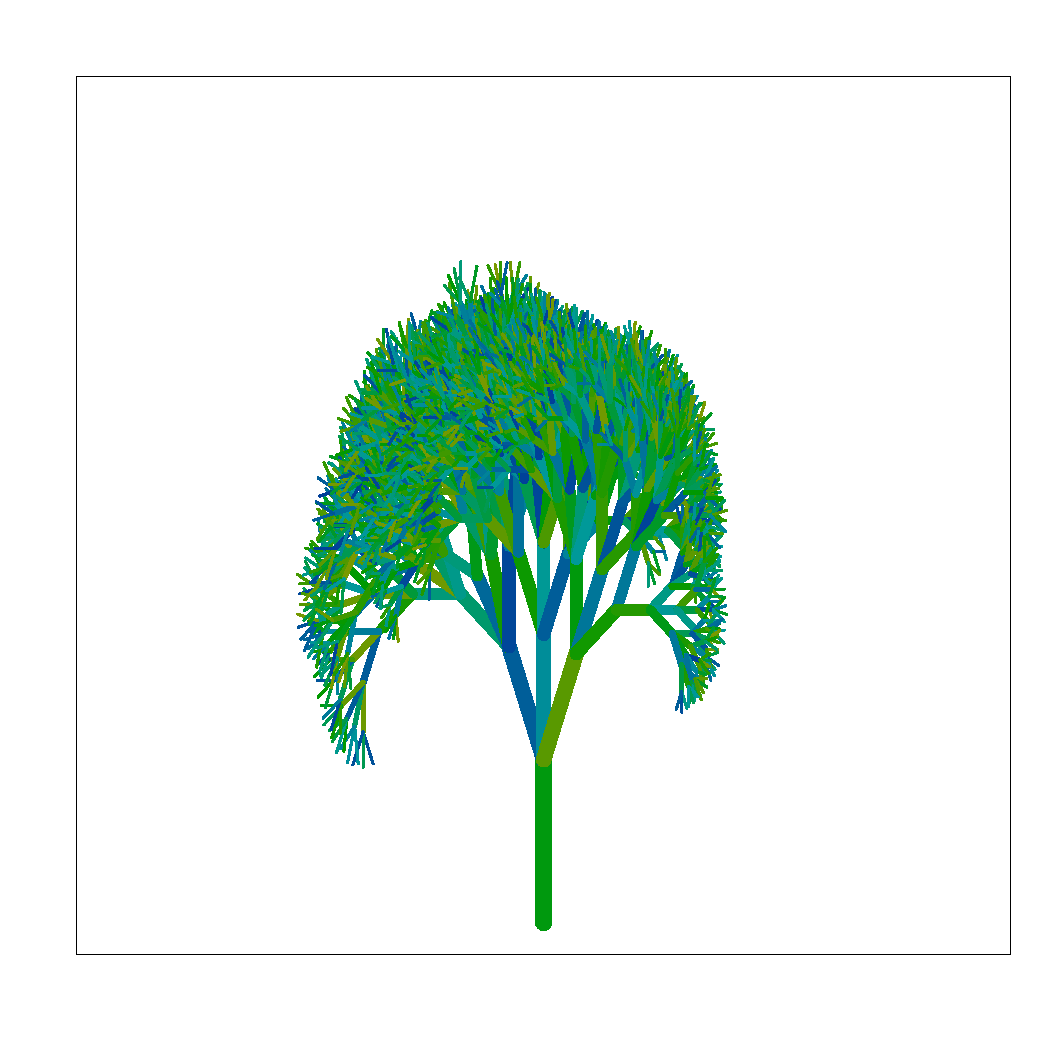
\includegraphics[width=0.5\textwidth]{figure/rectree-1} 

}



\end{knitrout}

\begin{knitrout}
\definecolor{shadecolor}{rgb}{0.969, 0.969, 0.969}\color{fgcolor}\begin{kframe}
\begin{alltt}
\hlstd{tree}\hlkwb{<-}\hlkwa{function}\hlstd{(}\hlkwc{x}\hlstd{,}\hlkwc{y}\hlstd{,}\hlkwc{l}\hlstd{,}\hlkwc{dir}\hlstd{,}\hlkwc{n}\hlstd{,}\hlkwc{nmax}\hlstd{)\{} \hlcom{# We define a function 'tree()'}
  \hlcom{# x,y: start of tree, l: length of first branch, dir: direction}
  \hlcom{# n and nmax: should be the same number: number of levels in the}
  \hlcom{# tree.}

  \hlcom{# An important escape argument, leave this out and the function}
  \hlcom{# will run forever:}
  \hlkwa{if}\hlstd{(n}\hlopt{==}\hlnum{0}\hlstd{)\{}
    \hlkwd{return}\hlstd{()}
  \hlstd{\}}

  \hlcom{# Picking a colour at random using the rainbow function}
  \hlcom{# (without this the code would also work, there would just be}
  \hlcom{# no colors)}
  \hlstd{pos}\hlkwb{<-}\hlkwd{round}\hlstd{(}\hlkwd{runif}\hlstd{(}\hlnum{1}\hlstd{,}\hlnum{1}\hlstd{,}\hlnum{199}\hlstd{))}
  \hlstd{colour}\hlkwb{=}\hlkwd{rainbow}\hlstd{(}\hlnum{200}\hlstd{,}\hlkwc{start}\hlstd{=}\hlnum{0.2}\hlstd{,}\hlkwc{end}\hlstd{=}\hlnum{0.6}\hlstd{,}\hlkwc{v}\hlstd{=}\hlnum{0.6}\hlstd{)[pos]}

  \hlcom{# Draw a line starting a (x,y) with length 'l' and in direction}
  \hlcom{# (in radials) dir. On top of that, we make the width of the }
  \hlcom{# line depend on how far the branch is from the stem.}
  \hlkwd{lines}\hlstd{(}\hlkwd{c}\hlstd{(x,x}\hlopt{+}\hlstd{l}\hlopt{*}\hlkwd{sin}\hlstd{(dir)),}\hlkwd{c}\hlstd{(y,y}\hlopt{+}\hlstd{l}\hlopt{*}\hlkwd{cos}\hlstd{(dir)),}
        \hlkwc{lwd}\hlstd{=}\hlnum{20}\hlopt{*}\hlstd{(n}\hlopt{/}\hlstd{nmax),}\hlkwc{col}\hlstd{=colour)}

  \hlcom{# Generate a random number that defines how many branches the }
  \hlcom{# tree has at this point in the structure}
  \hlstd{branches}\hlkwb{<-}\hlkwd{round}\hlstd{(}\hlkwd{runif}\hlstd{(}\hlnum{1}\hlstd{,}\hlnum{2}\hlstd{,}\hlnum{4}\hlstd{))}

  \hlcom{# Now we go over the separate branches}
  \hlkwa{for}\hlstd{(i} \hlkwa{in} \hlnum{1}\hlopt{:}\hlstd{branches)\{}
    \hlcom{# to make sure not all branches point in the same direction,}
    \hlcom{# we calculate a direction for the branch}
    \hlstd{angle}\hlkwb{<-}\hlstd{dir}\hlopt{+}\hlstd{(}\hlopt{-}\hlstd{pi}\hlopt{/}\hlnum{6}\hlstd{)}\hlopt{+}\hlstd{(pi}\hlopt{/}\hlnum{3}\hlstd{)}\hlopt{*}\hlstd{(i}\hlopt{-}\hlnum{1}\hlstd{)}\hlopt{/}\hlstd{(branches}\hlopt{-}\hlnum{1}\hlstd{)}

    \hlcom{# Also, we would like the later branches to be smaller than}
    \hlcom{# the first one:}
    \hlstd{l2}\hlkwb{<-}\hlkwd{runif}\hlstd{(}\hlnum{1}\hlstd{,}\hlnum{0.7}\hlstd{,}\hlnum{0.85}\hlstd{)}\hlopt{*}\hlstd{l}

    \hlcom{# And finally the magic of recursion, we draw the new branch}
    \hlcom{# simply by using theexact same function: the function 'tree'.}
    \hlkwd{tree}\hlstd{(x}\hlopt{+}\hlstd{l}\hlopt{*}\hlkwd{sin}\hlstd{(dir),y}\hlopt{+}\hlstd{l}\hlopt{*}\hlkwd{cos}\hlstd{(dir),l2,angle,n}\hlopt{-}\hlnum{1}\hlstd{,nmax)}
  \hlstd{\}}
\hlstd{\}}

\hlcom{# Now, to actually draw the tree, we first make an empty plot}
\hlkwd{plot}\hlstd{(}\hlnum{0}\hlstd{,}\hlnum{0}\hlstd{,}\hlkwc{type}\hlstd{=}\hlstr{"n"}\hlstd{,}\hlkwc{xlim}\hlstd{=}\hlkwd{c}\hlstd{(}\hlopt{-}\hlnum{10}\hlstd{,}\hlnum{10}\hlstd{),}\hlkwc{ylim}\hlstd{=}\hlkwd{c}\hlstd{(}\hlnum{0}\hlstd{,}\hlnum{10}\hlstd{),}
     \hlkwc{xaxt}\hlstd{=}\hlstr{"n"}\hlstd{,}\hlkwc{yaxt}\hlstd{=}\hlstr{"n"}\hlstd{,}\hlkwc{ylab}\hlstd{=}\hlstr{""}\hlstd{,}\hlkwc{xlab}\hlstd{=}\hlstr{""}\hlstd{)}

\hlcom{# And then call the function tree() with the parameters we like}
\hlkwd{tree}\hlstd{(}\hlnum{0}\hlstd{,}\hlnum{0}\hlstd{,}\hlnum{2}\hlstd{,}\hlnum{0}\hlstd{,}\hlnum{8}\hlstd{,}\hlnum{8}\hlstd{)}
\end{alltt}
\end{kframe}
\end{knitrout}
\end{document}
